\chapter{Finalisation et réalisation de la canne}

\section{Les étapes de la réalisation d'un circuit imprimé}
\label{realisation-circuit-imprime}

\subsection{Découpe}
Découpe à la cisaille d'une plaque de la taille du circuit à réaliser, suppression de l'adhésif de protection.

\subsubsection*{Cisaille guillotine}
Cisaille guillotine de capacité de coupe de 380mm équipée de lames en acier spécial étudiées pour la coupe des matériaux employés dans la fabrication des circuit imprimes (XXXF, VERRE EPOXY). \\
Cette machine peut-être aussi utlisee pour la coupe des materiaux comme:
\begin{itemize}
    \item L'aluminium
    \item Cuivre
    \item Laiton
    \item Acier
    \item $\hdots$
\end{itemize}
Cette machine est équipée d'une butée d'angle et d'une butée arrière réglable pour découpe en série.

\paragraph*{Caractéristiques techniques}
\begin{itemize}
    \item Largeur de coupe: 380mm
    \item Longueur butée arrière: 175mm
    \item Dimensions: 620 x 430 x 450 mm
    \item Poids: 45Kg
\end{itemize}

\paragraph*{Capacité de coupe}
\begin{itemize}
    \item Tète acier doux: 1.2mm
    \item Tète aluminium: 1.5mm
    \item Stratifiés: 1.6mm
\end{itemize}


\subsection{Insolation}
Positionnement de la plaque et du calque dans l'insoleuse. Ils sont maintenus par le vide pendant l'exposition aux rayons ultras-violets
\paragraph*{Durée d'insolation} 3mn

\begin{figure}[!htbp]
    \centering
    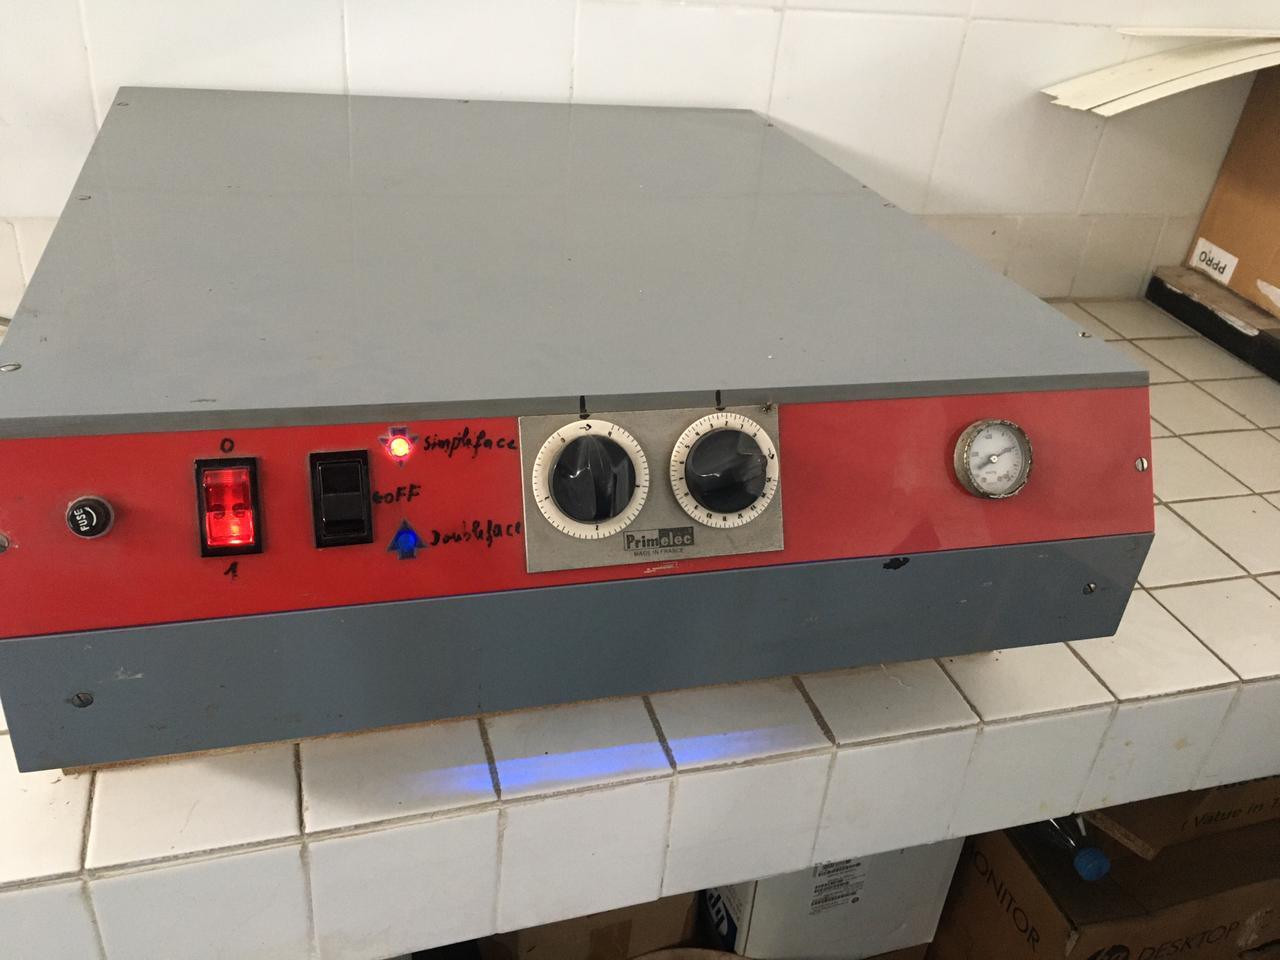
\includegraphics[width=.7\linewidth]{assets/realisation/x4.jpeg}
    \caption{Châssis d'insolation}
\end{figure}

\FloatBarrier

\subsection{Immersion}
Immersion de la plaque pendant 2 min dans bain de révélateur. \\
Rinçage abondant à l'eau courante pour stopper l'action du révélateur. \\
Seules les parties non exposées aux U.V restent protégées par la couche photosensible. \\
Le révélateur utilisé (hydrate de soude) est livré en granules. \\
Dissolver le contenu d'un sachet dans un litre d'eau (max: 25$^{\circ}$C). \\
Il doit toujours être remis immédiatement en bouteille après utilisation (Altération à l'air).

\subsection{Gravure}
Par projection de perchlorure de fer pour éliminer le cuivre non protégée.
Durée de gravure environ 5 minutes. \\
Rinçage très abondant de l'eau courant.
\begin{itemize}
    \item {\color{red} Attention:} le perchlorure de fer est un produit dangereux (acide)
    \item {\color{red} Attention:} aux projections (yeux, habits, $\hdots$). Mettez une blouse et des lunettes de protection!
\end{itemize}

\begin{figure}[!htbp]
    \centering
    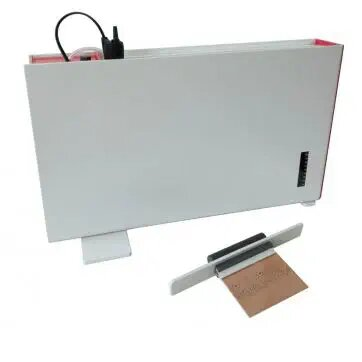
\includegraphics[width=.7\linewidth]{assets/realisation/graveuse.jpg}
    \caption{Graveuse CIF bb4}
\end{figure}

\FloatBarrier

\subsection{Nettoyage}
Élimination de la couche de protection avec un tampon imbibé d'alcool.

\subsection{Perçage}
Forêt carbure a partir de diamètre 0.5mm.
Vitesse de rotation:  15000 à 20000 Tr/min \\
Forêt acier rapide à partir de diamètre 0.8mm.
Vitesse de rotation: 2250 à 3000 Tr/min

\begin{figure}[!htbp]
    \centering
    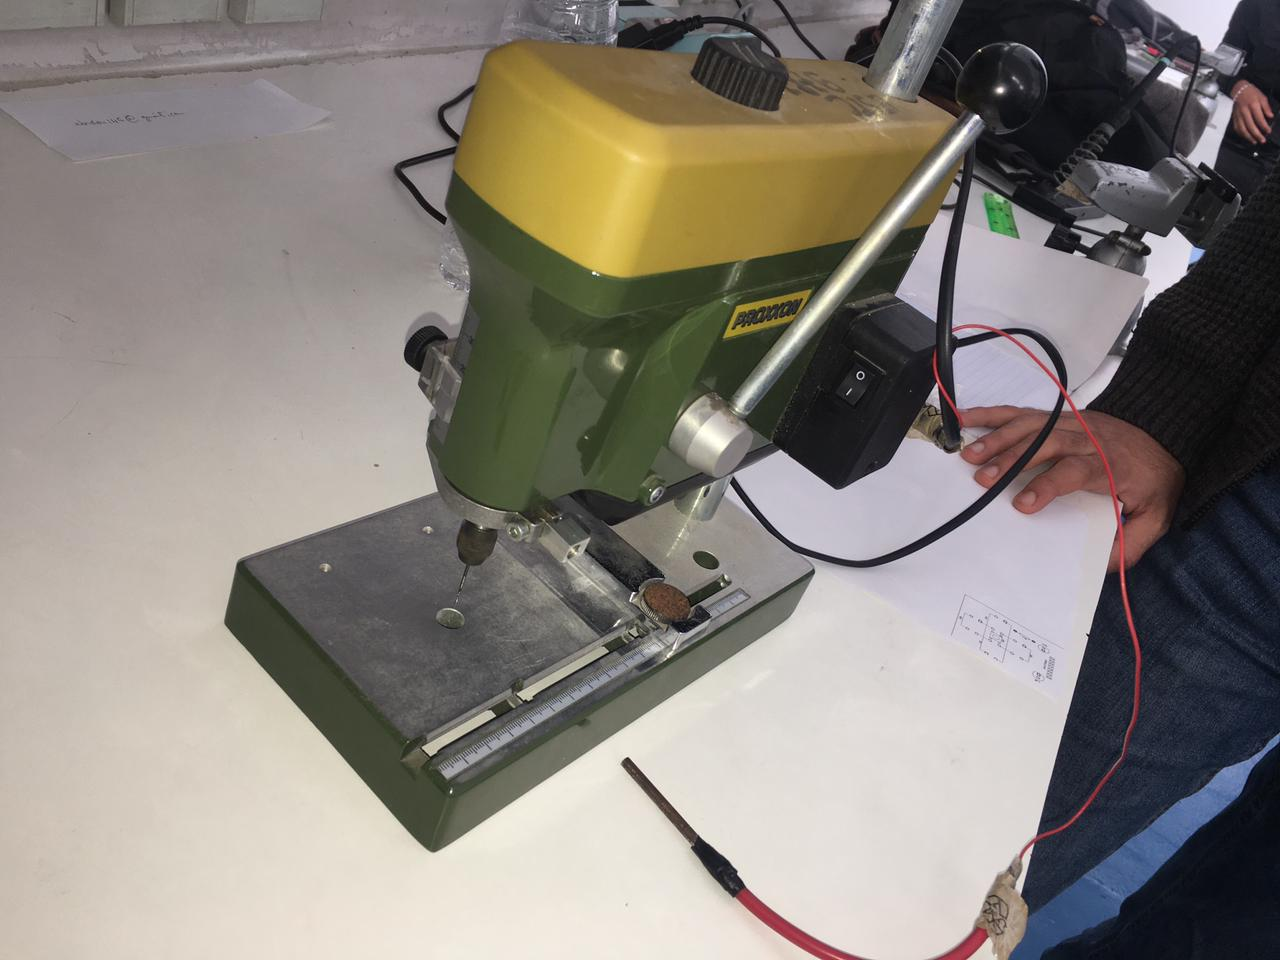
\includegraphics[width=.7\linewidth]{assets/realisation/x14.jpeg}
    \caption{Perceuse}
\end{figure}

\FloatBarrier

\section{PCB du circuit des boutons}
Après avoir faire la conception du circuit des boutons (Chapitre \ref{buttons-circuit-conception}), on doit maintenant le réaliser suivant les étapes expliquées précédemment (Chapitre \ref{realisation-circuit-imprime}).

Après la découpe, l'insolation et  (on manque les photos), on l'immerge:

\begin{figure}[!htbp]
    \centering
    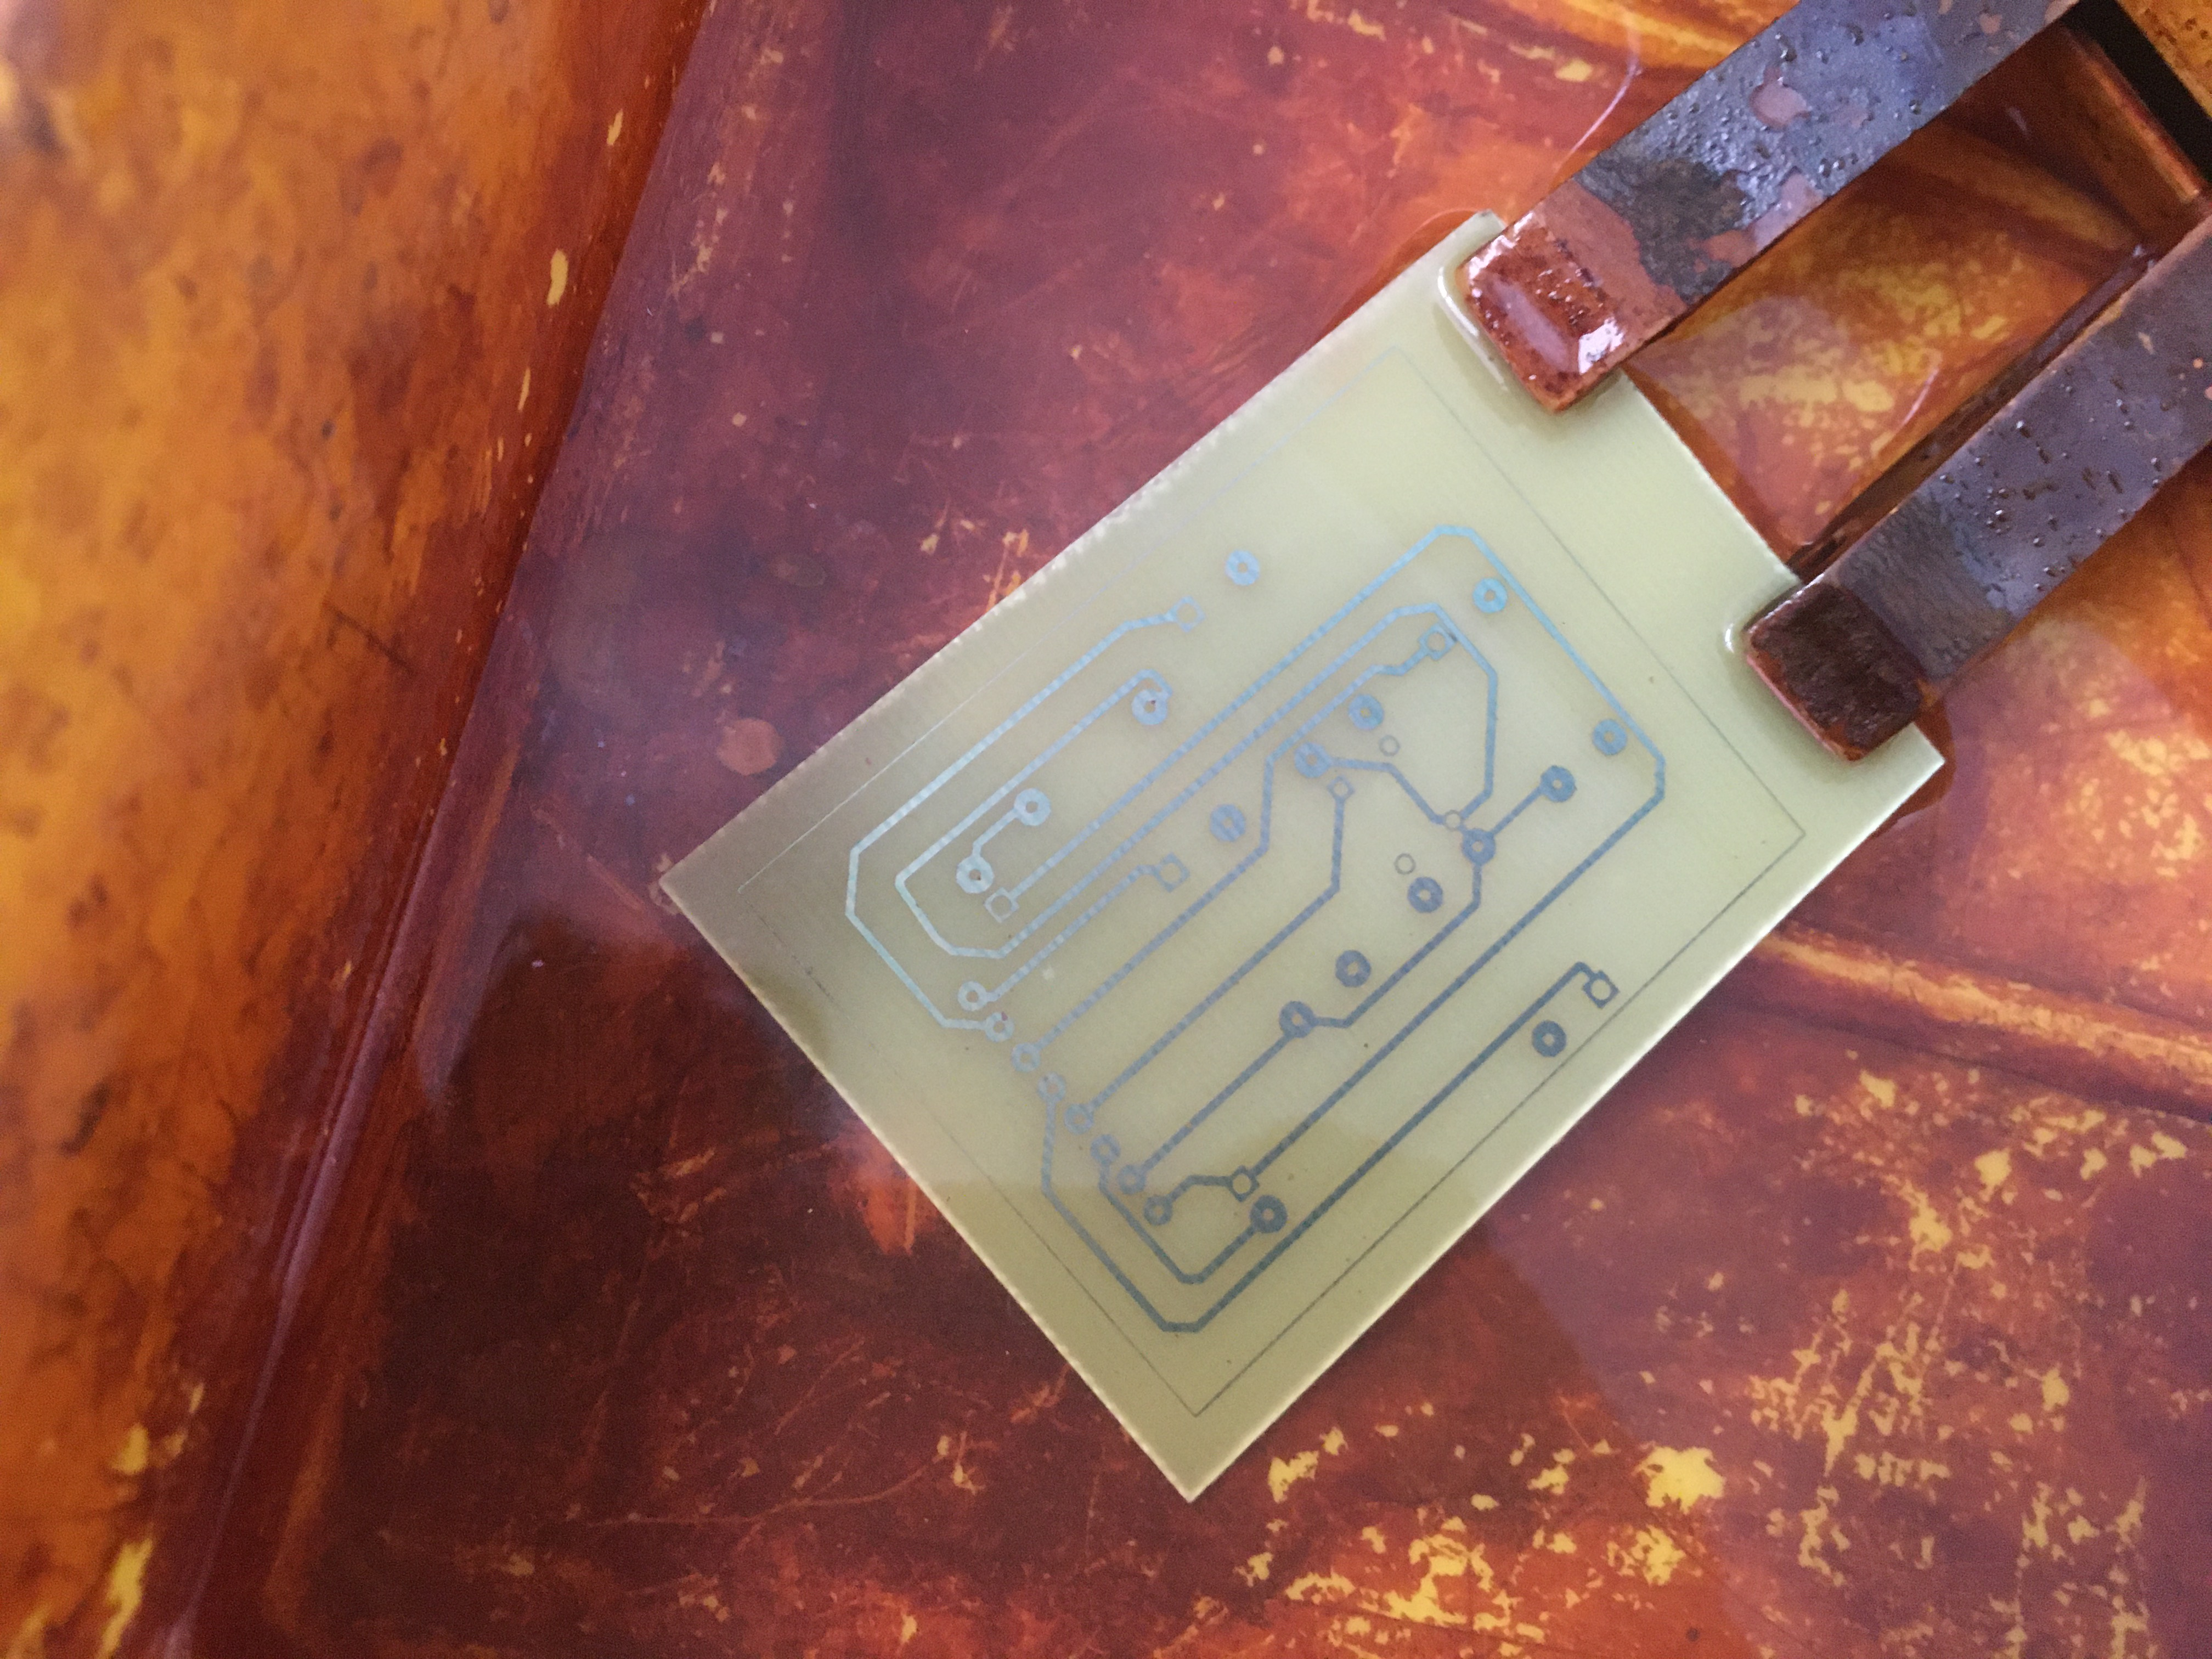
\includegraphics[width=.6\textwidth]{assets/realisation/cartes/2022-03-25 12.20.16.jpeg}
    \caption{L'immersion du circuit imprimé des boutons}
\end{figure}

\FloatBarrier

Puis on fait le perçage:

\begin{figure}[!htbp]
    \centering
    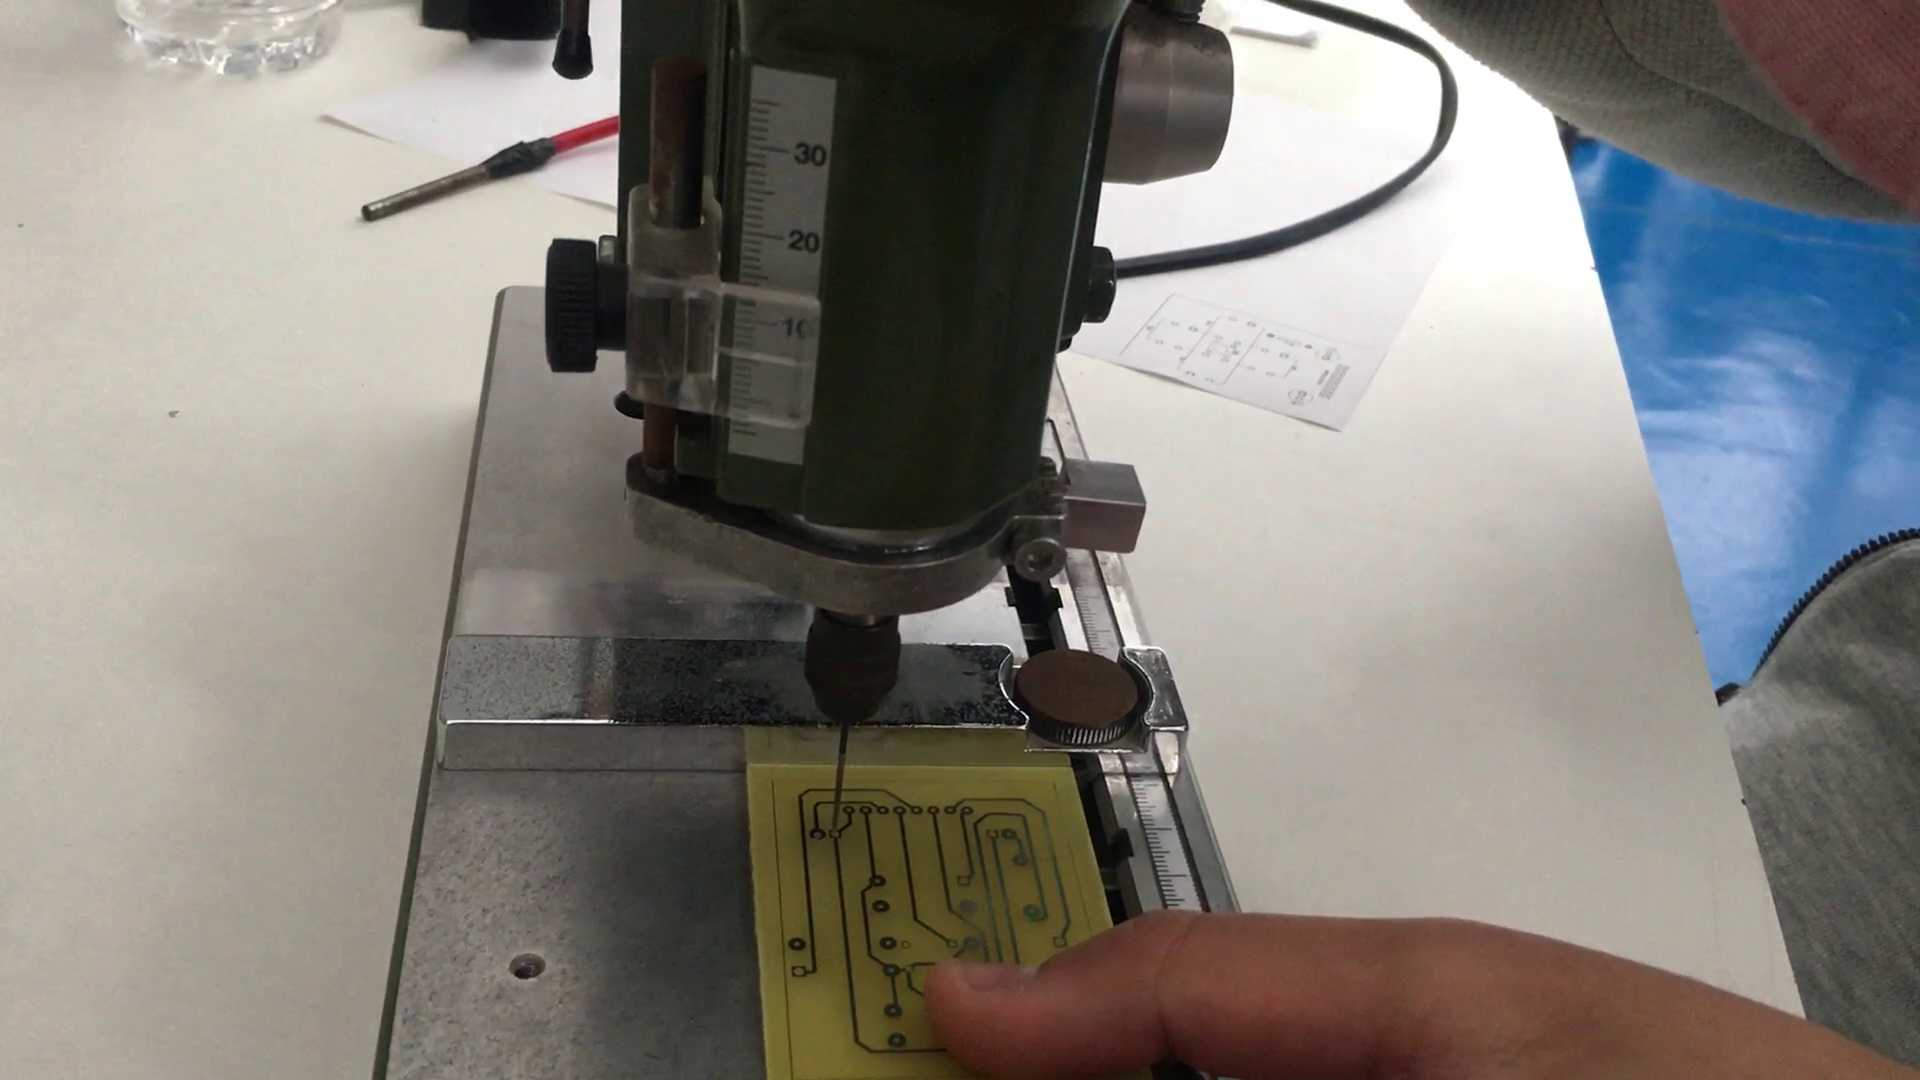
\includegraphics[width=\textwidth]{assets/realisation/cartes/vlcsnap-2022-04-14-04h43m27s441.png}
    \caption{Perçage du circuit imprimé des boutons}
\end{figure}

\FloatBarrier

Après, nous soudons les composant sur la carte:

\begin{figure}[!htbp]
    \centering
    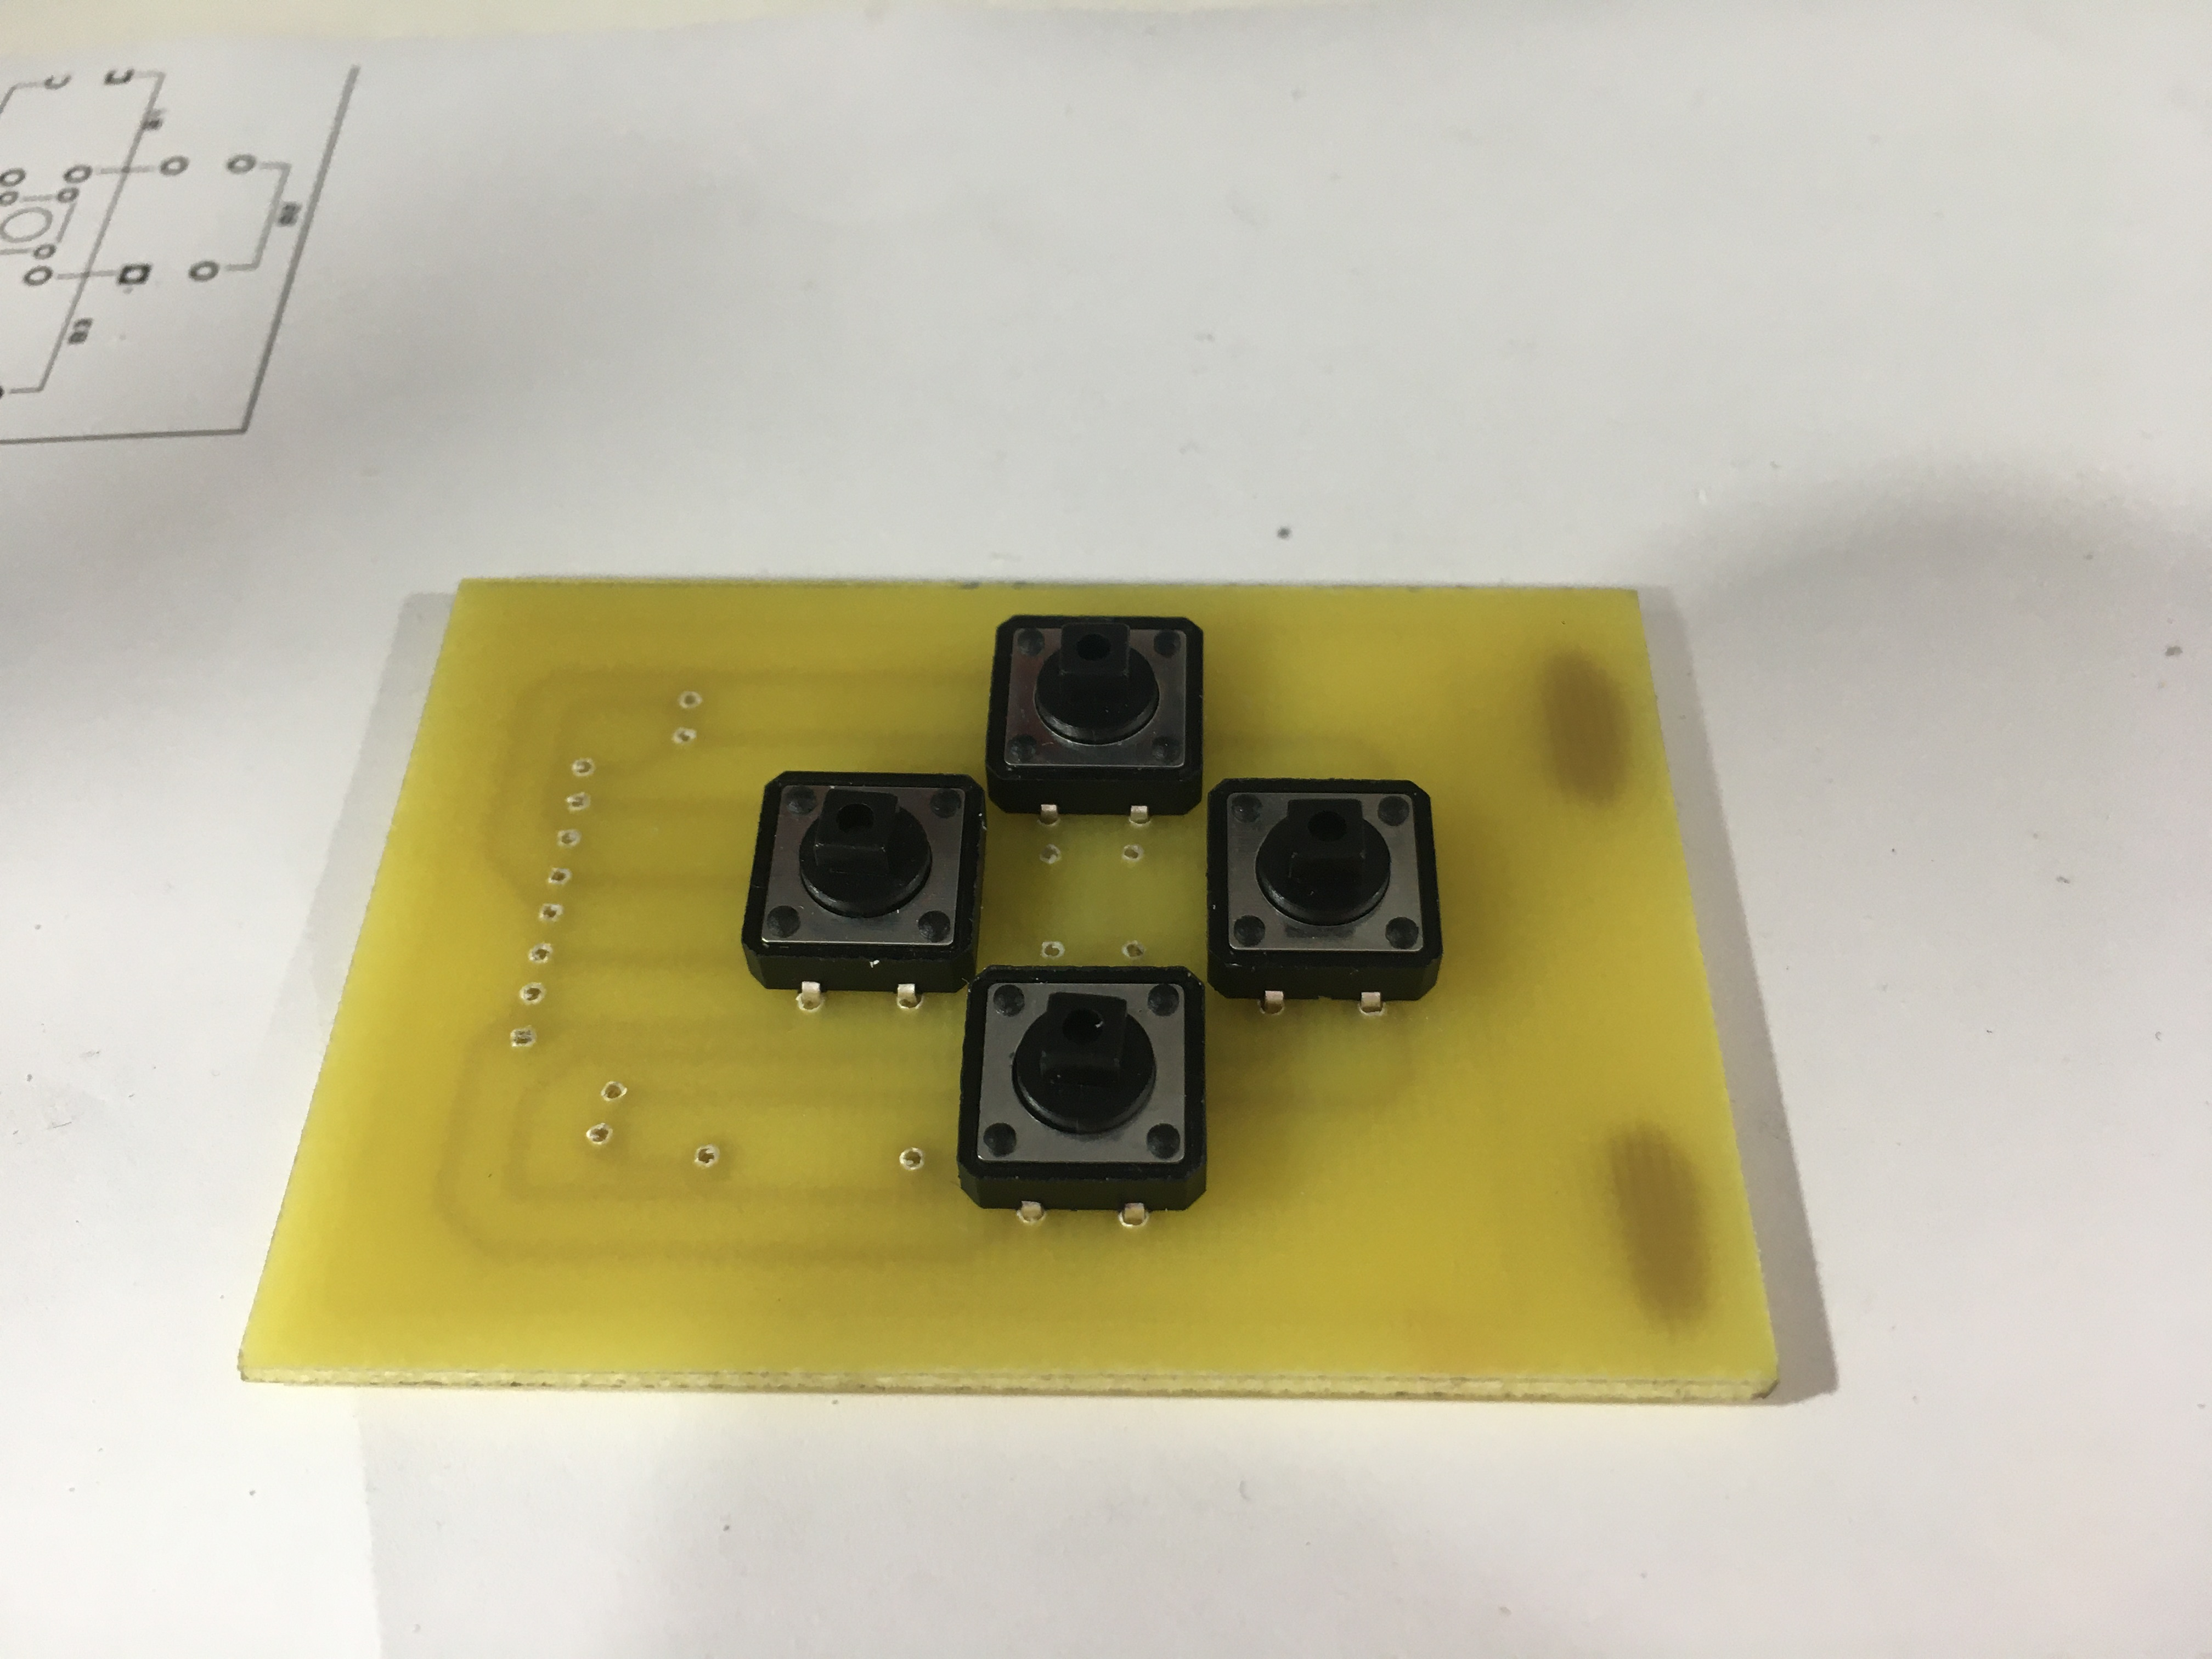
\includegraphics[width=.6\textwidth]{assets/realisation/cartes/2022-03-25 15.17.03.jpeg}
    \caption{Boutons soudés circuit imprimé des boutons}
\end{figure}

\FloatBarrier

Carte des boutons final:

\begin{figure}[!htbp]
    \centering
    \begin{subfigure}[m]{.31\linewidth}
        \centering
        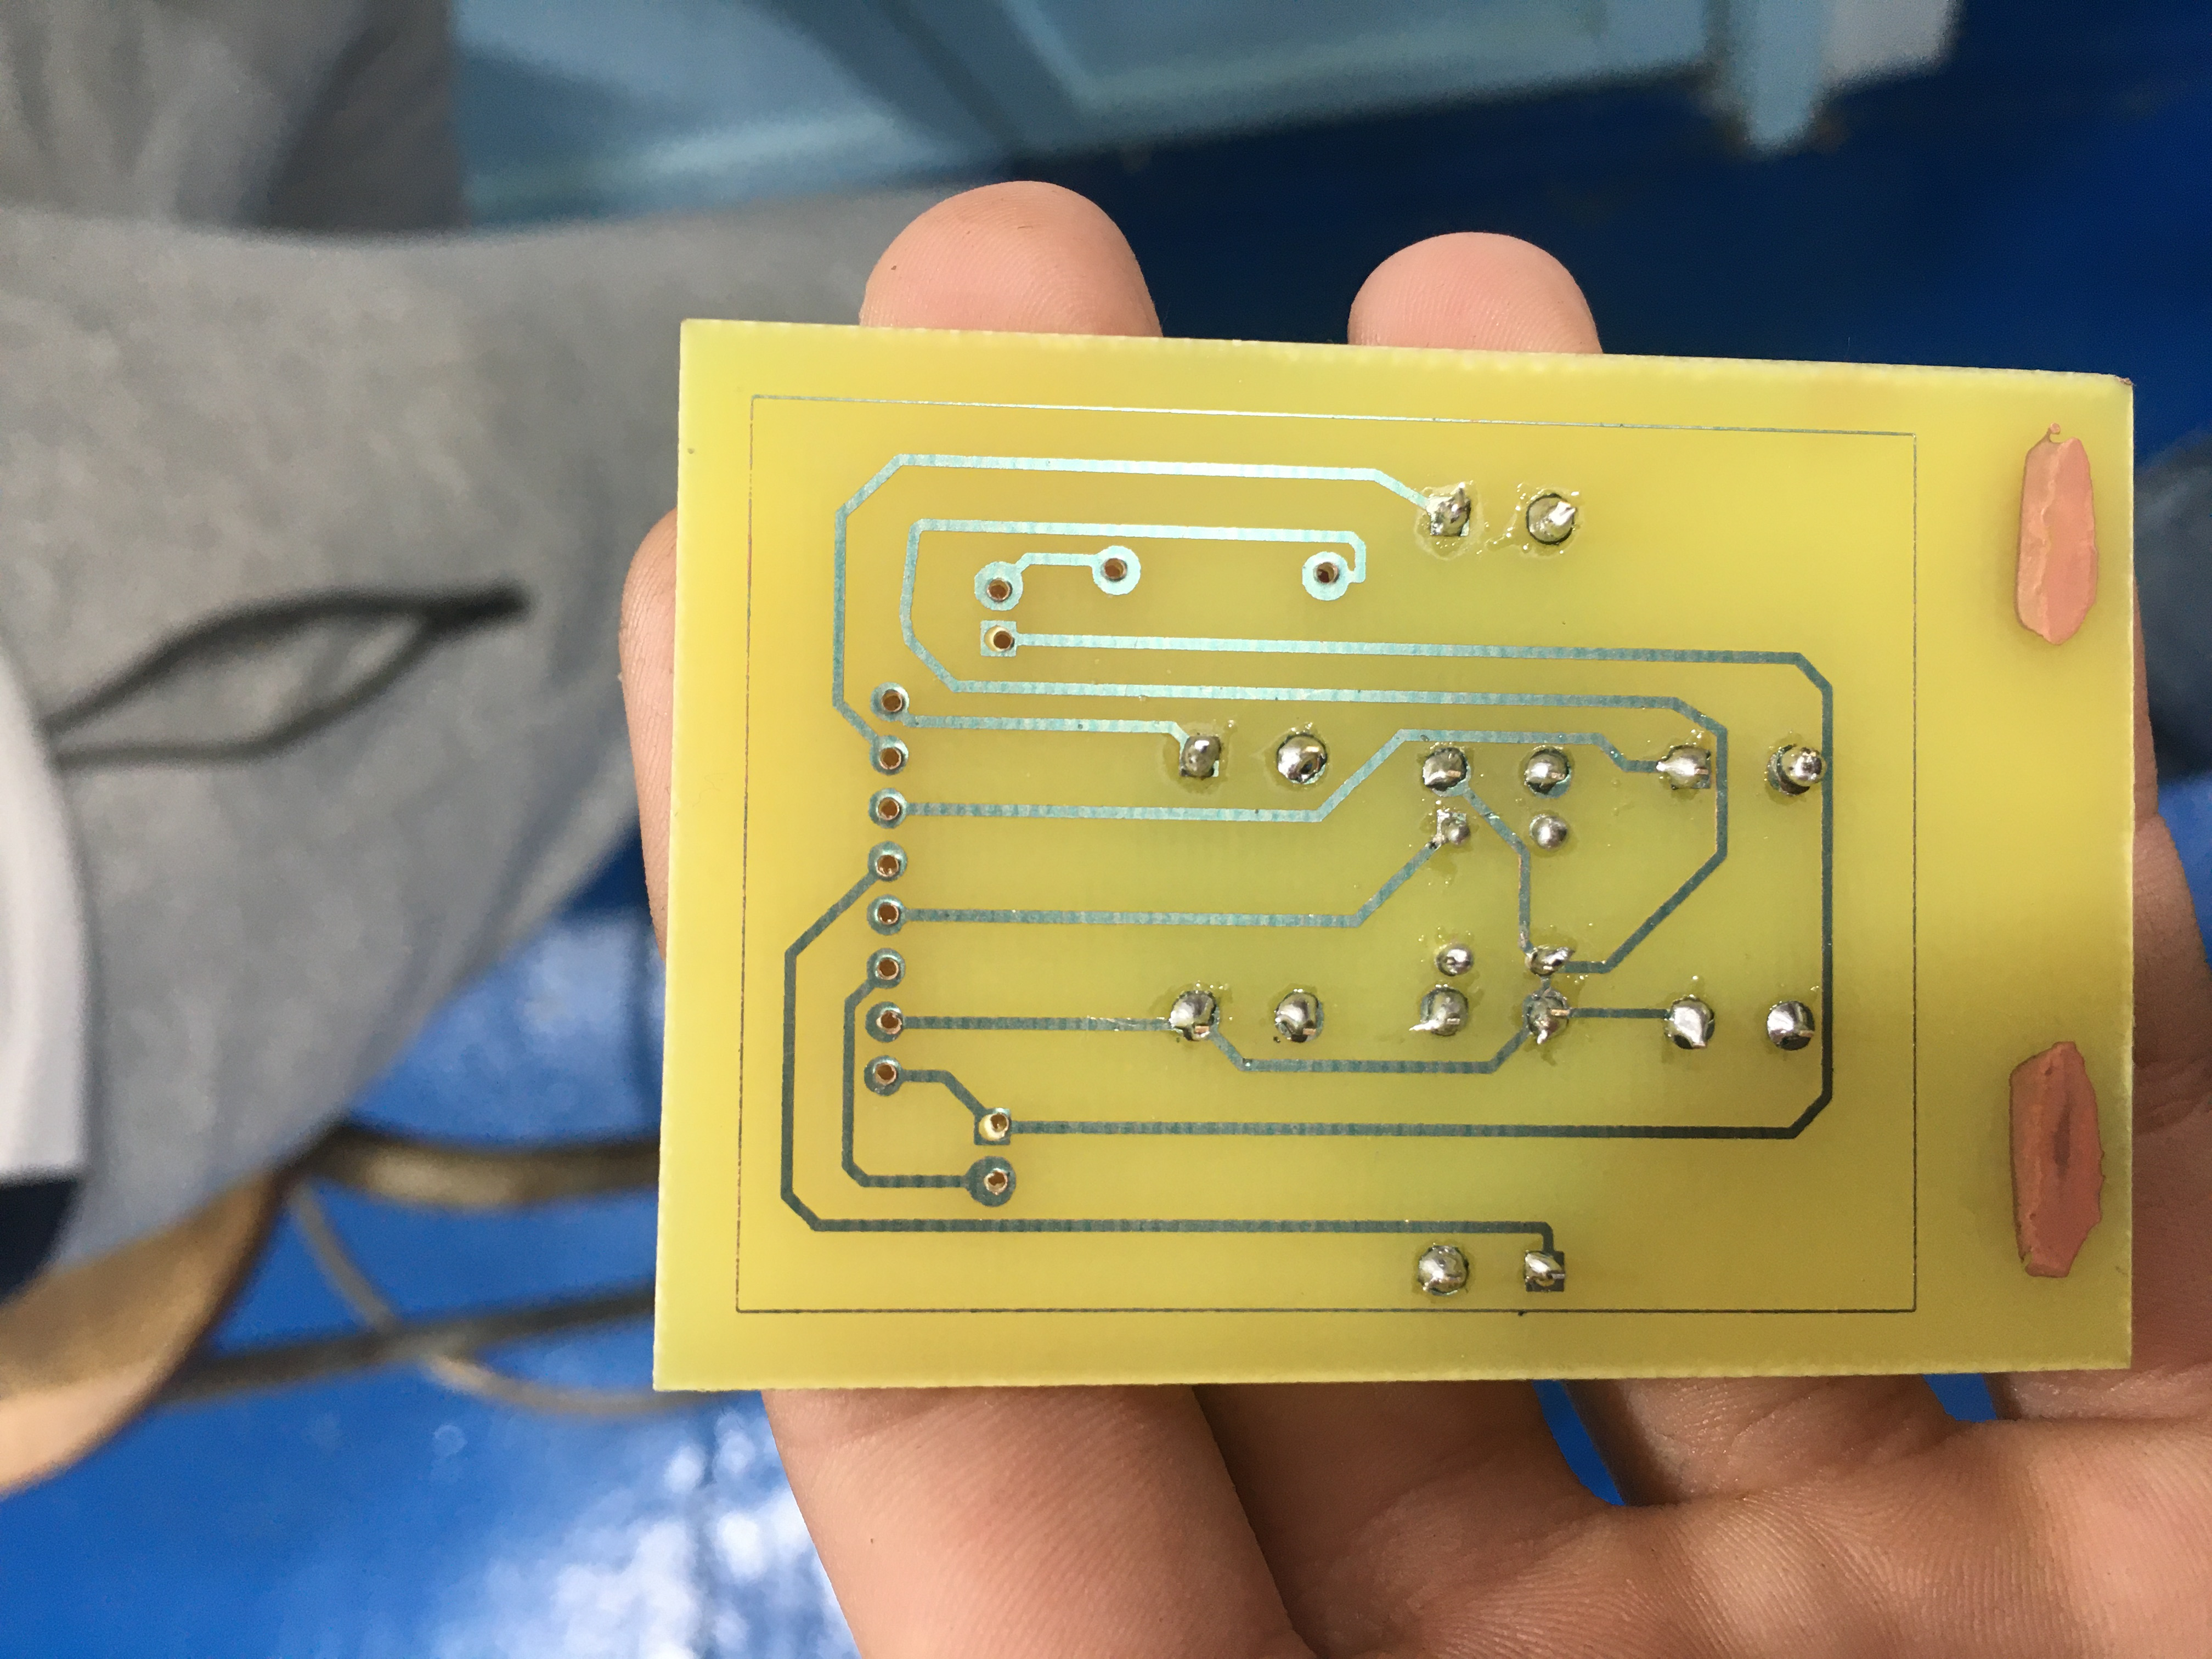
\includegraphics[width=\textwidth]{assets/realisation/cartes/2022-03-25 15.34.40.jpeg}
    \end{subfigure}
    \hfill
    \begin{subfigure}[m]{.31\linewidth}
        \centering
        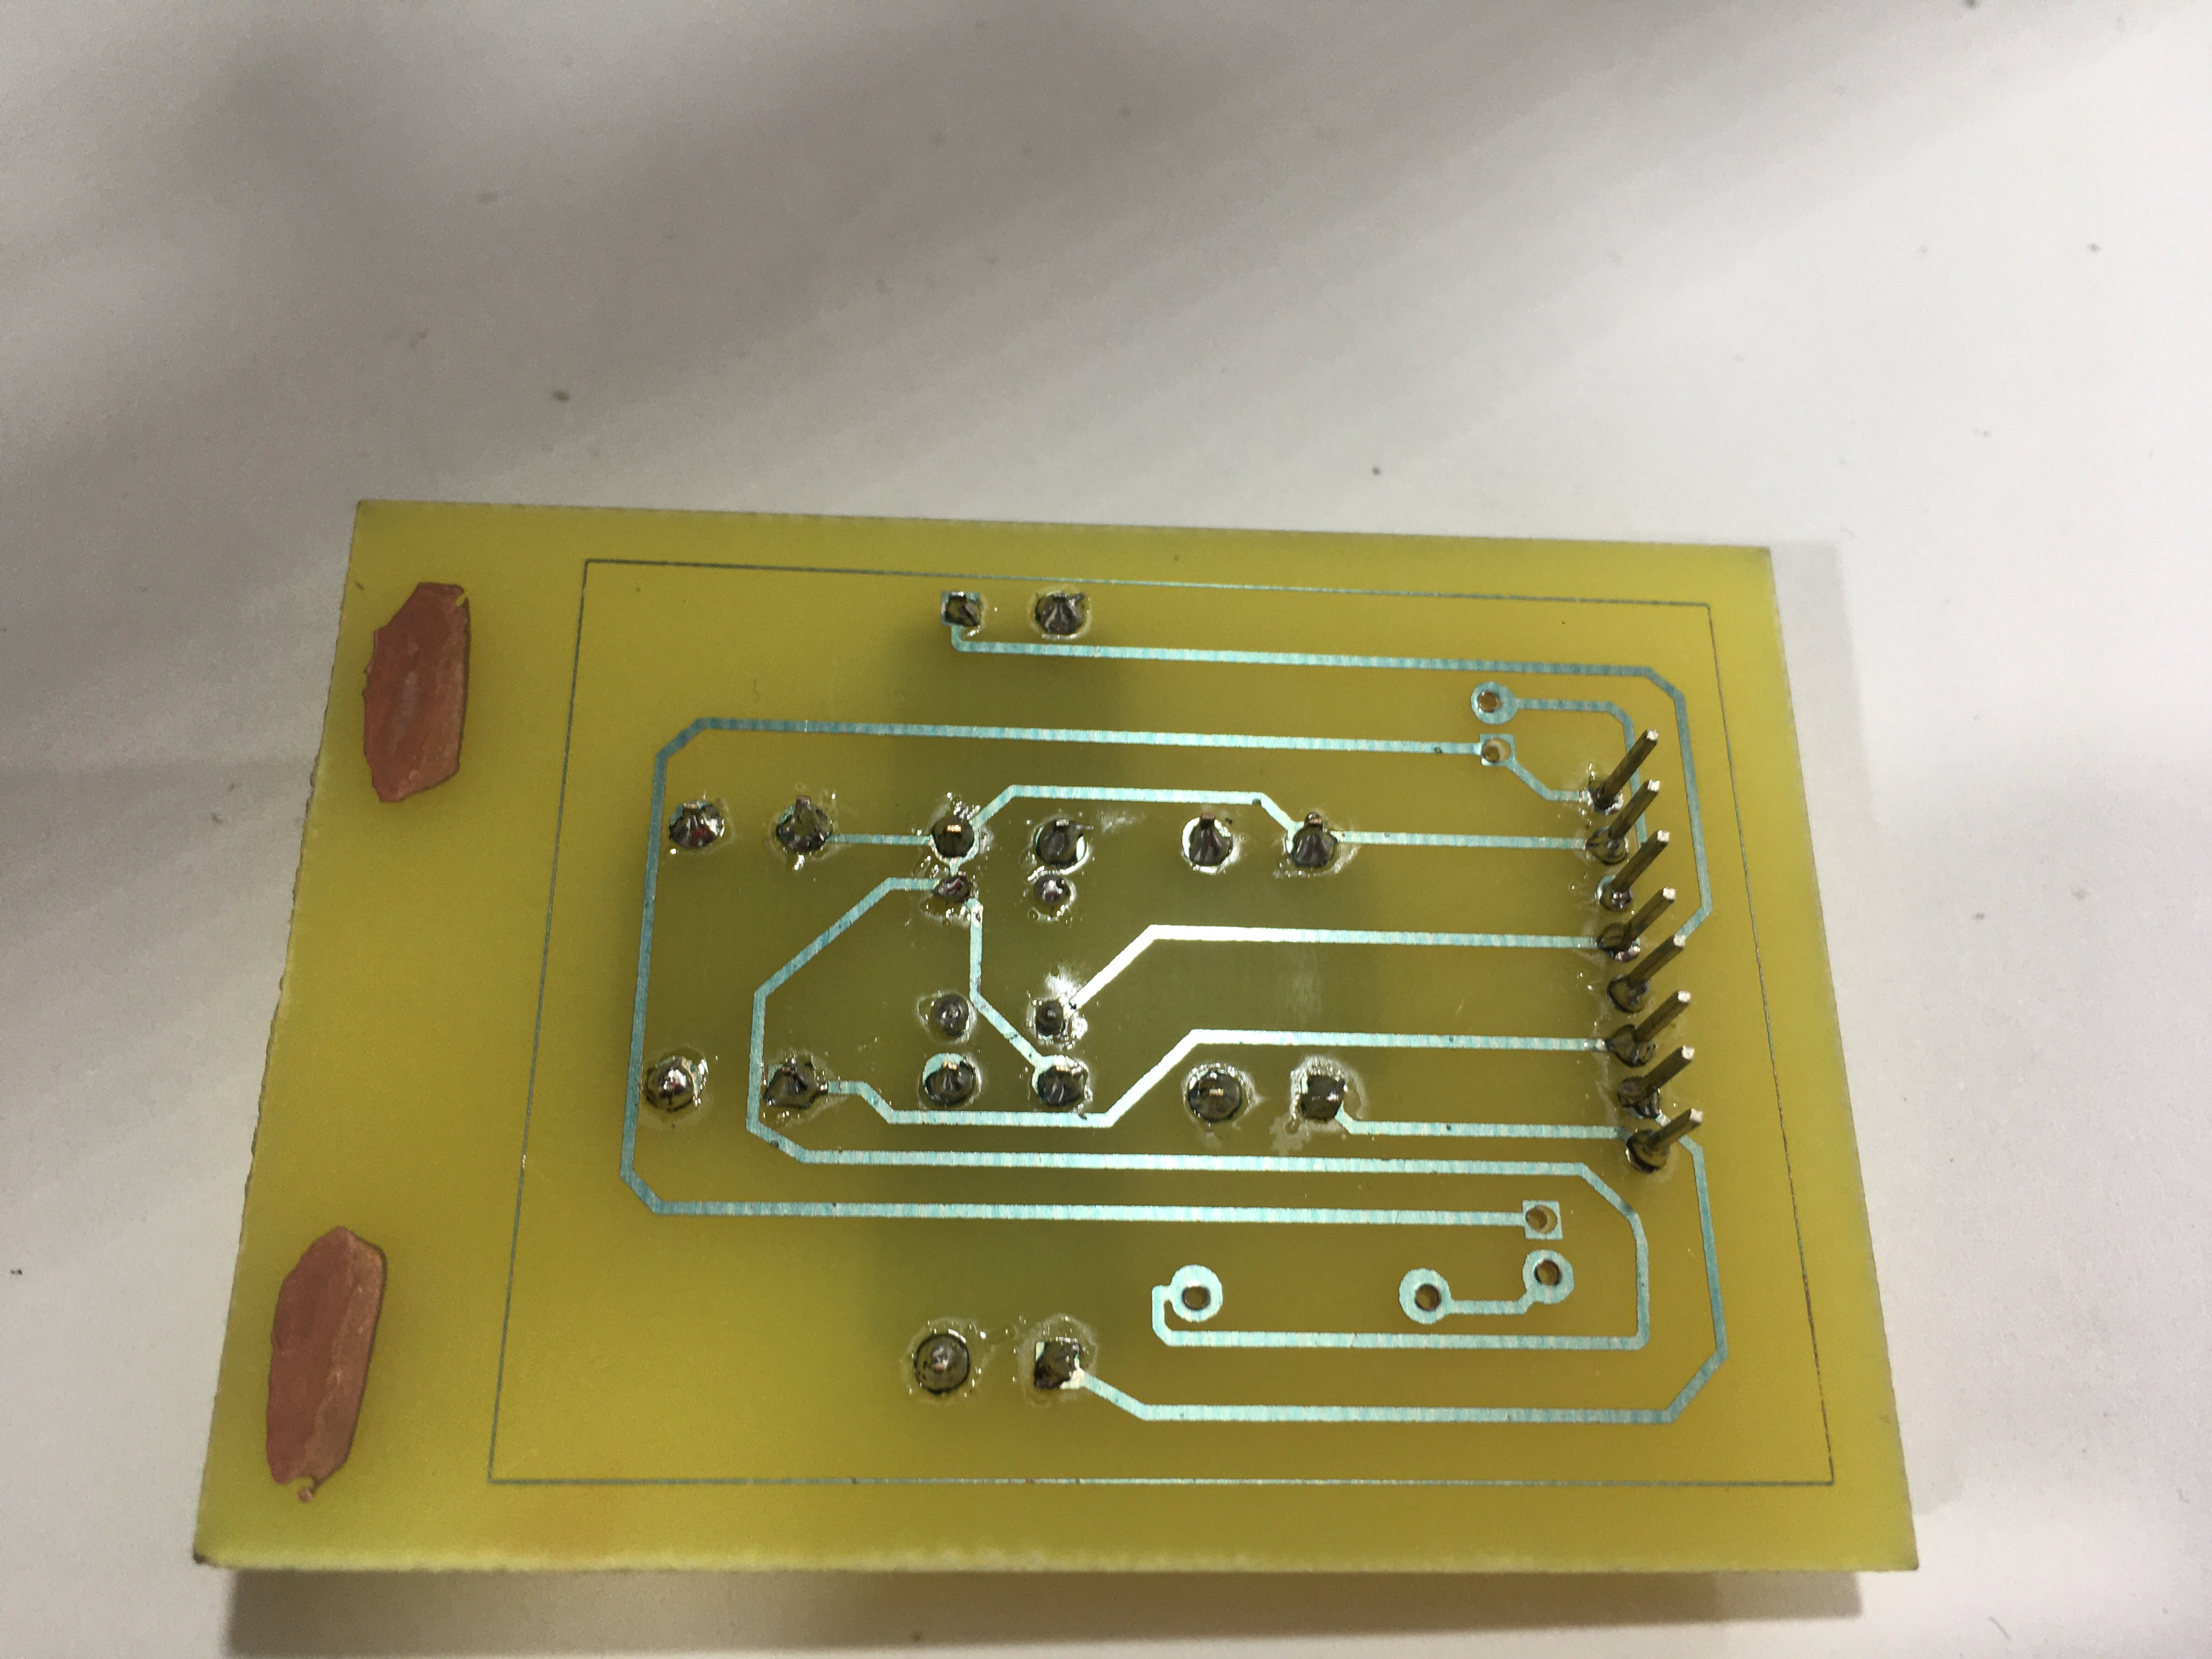
\includegraphics[width=\textwidth]{assets/realisation/cartes/2022-03-25 16.30.00.jpeg}
    \end{subfigure}
    \hfill
    \begin{subfigure}[m]{.31\linewidth}
        \centering
        \rotatebox[origin=c]{-90}{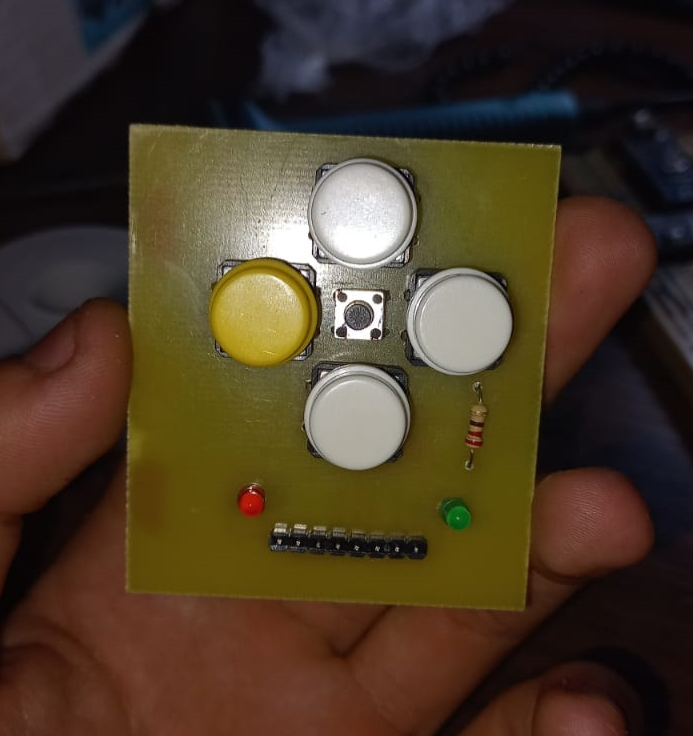
\includegraphics[height=\textwidth]{assets/realisation/cartes/2022-03-28 22.40.09.jpeg}}
    \end{subfigure}
    \caption{Circuit imprimé final des boutons}
\end{figure}

\FloatBarrier

\section{PCB du circuit Arduino}

\begin{figure}[!htbp]
    \centering
    \begin{subfigure}[m]{.23\linewidth}
        \centering
        \rotatebox[origin=c]{-90}{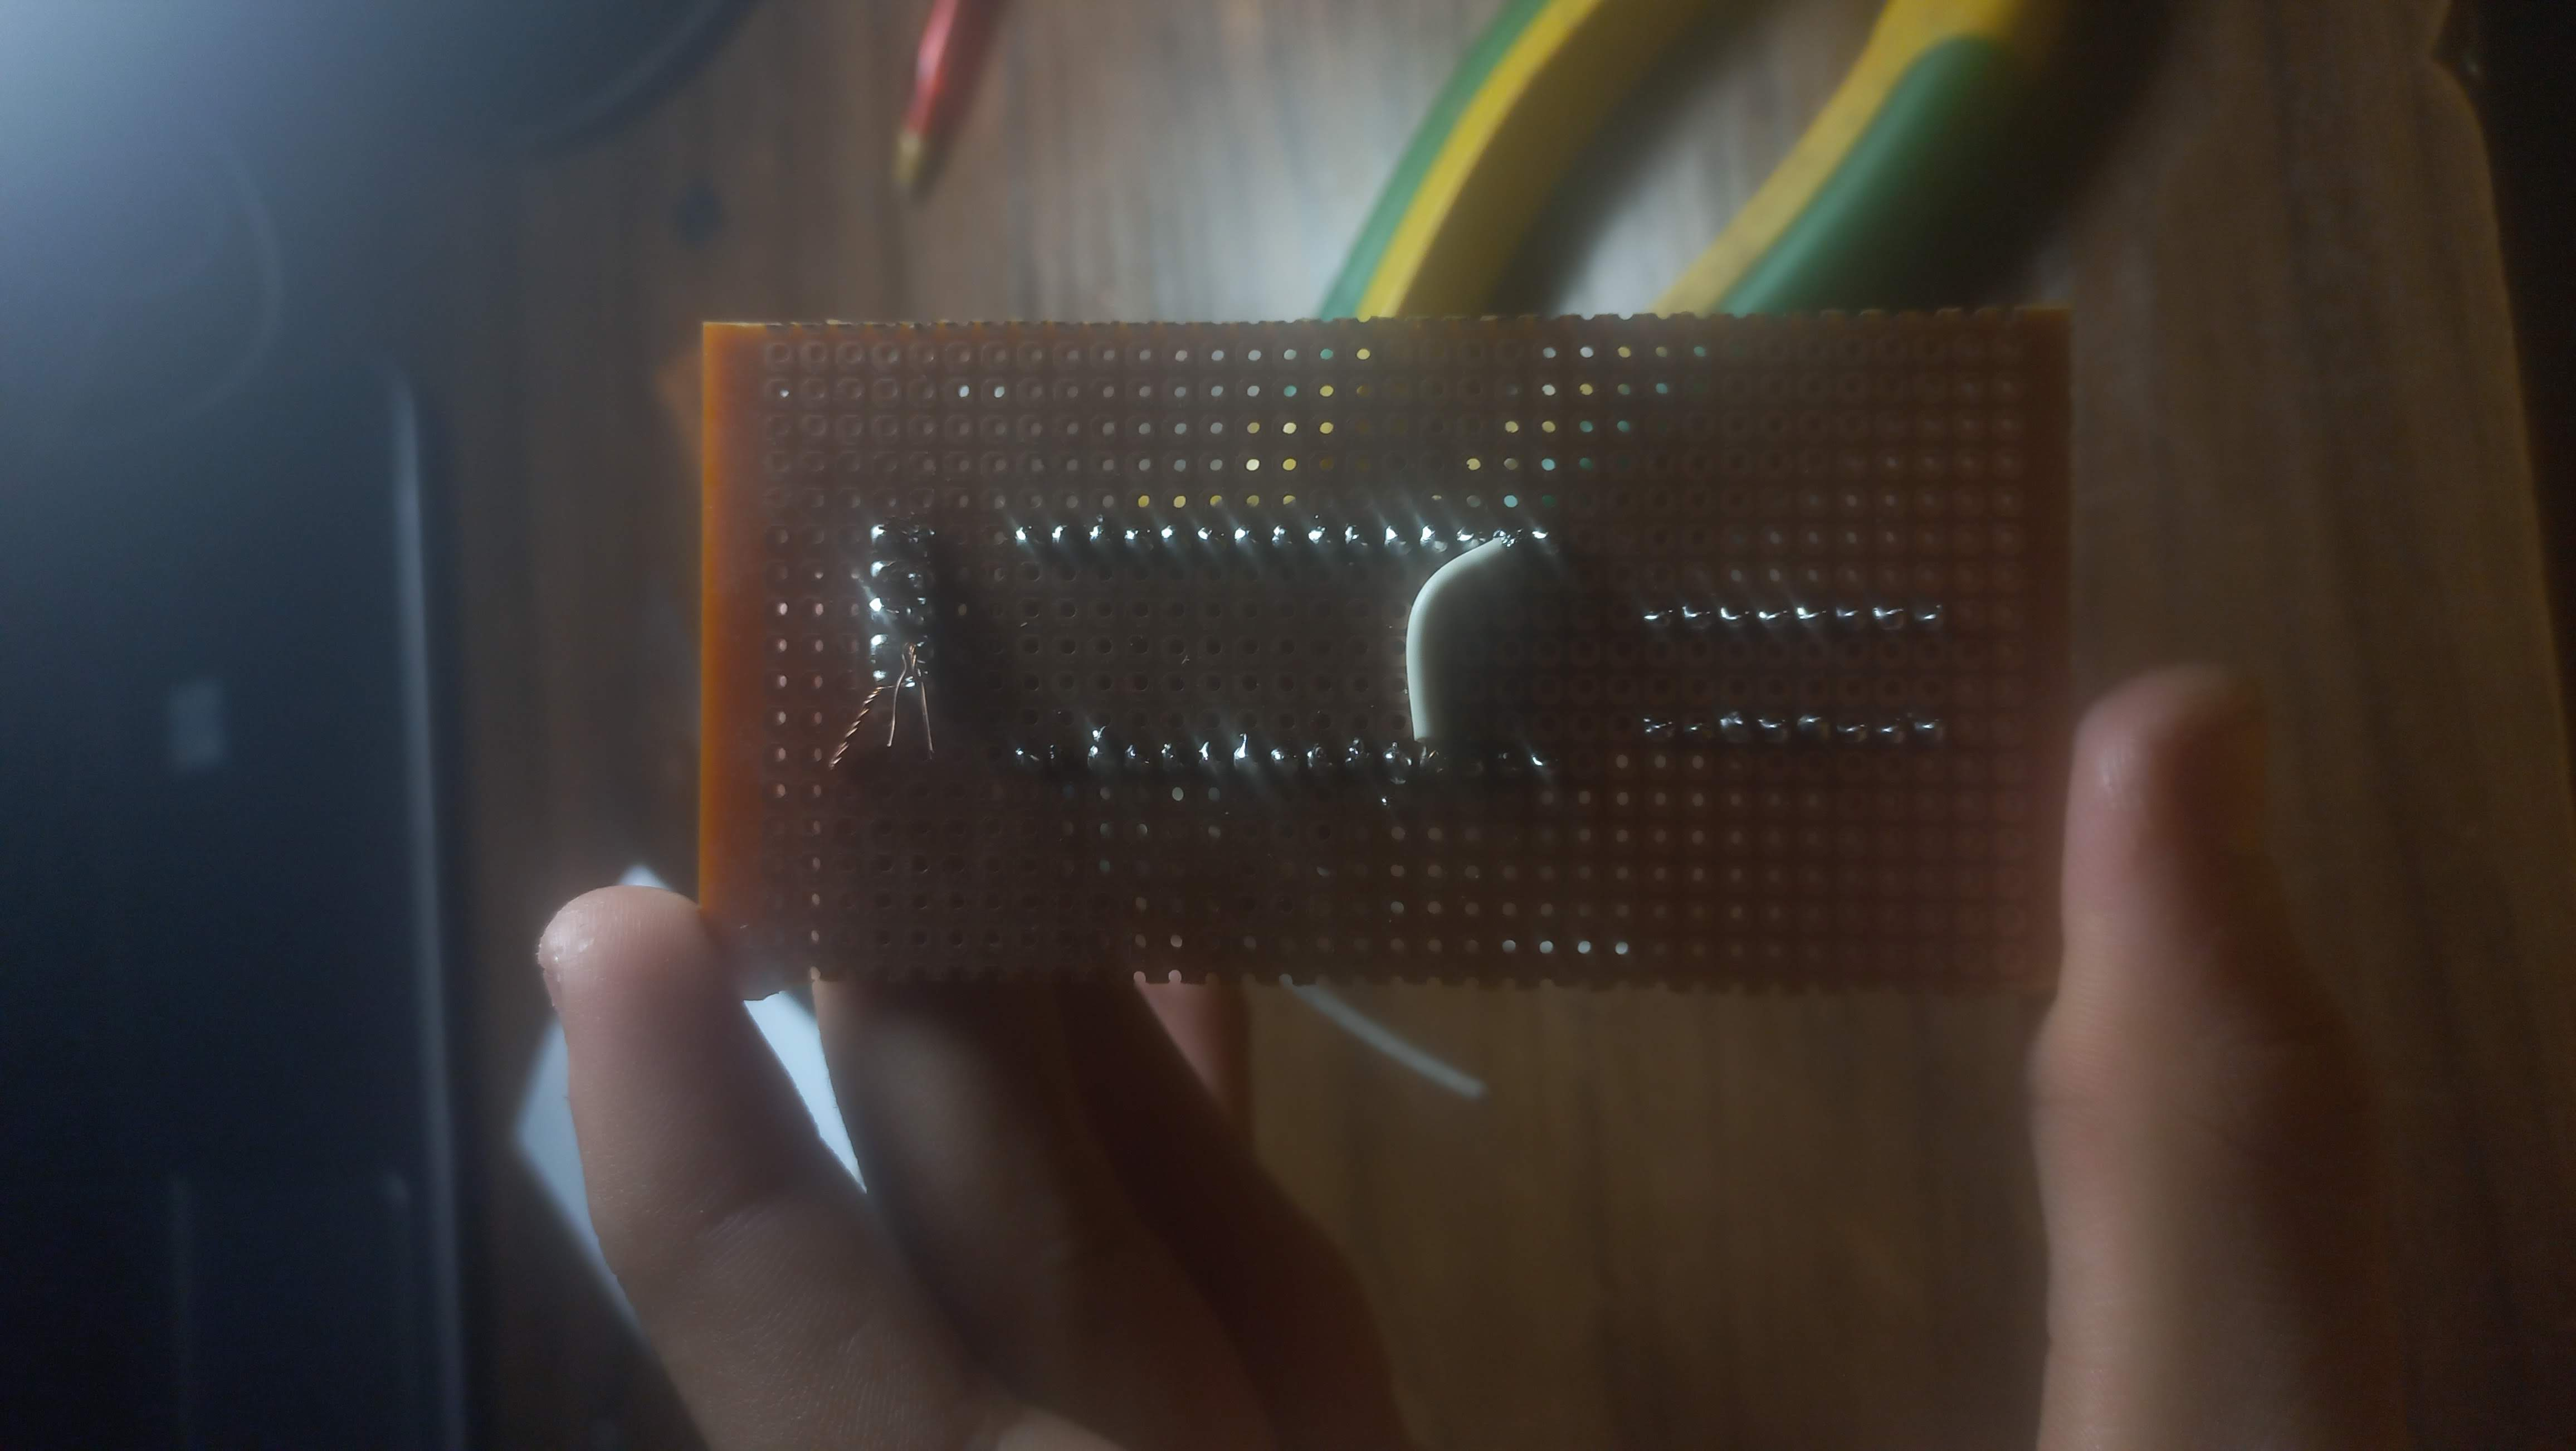
\includegraphics[height=\textwidth]{assets/realisation/1.jpg}}
    \end{subfigure}
    \hfill
    \begin{subfigure}[m]{.23\linewidth}
        \centering
        \rotatebox[origin=c]{-90}{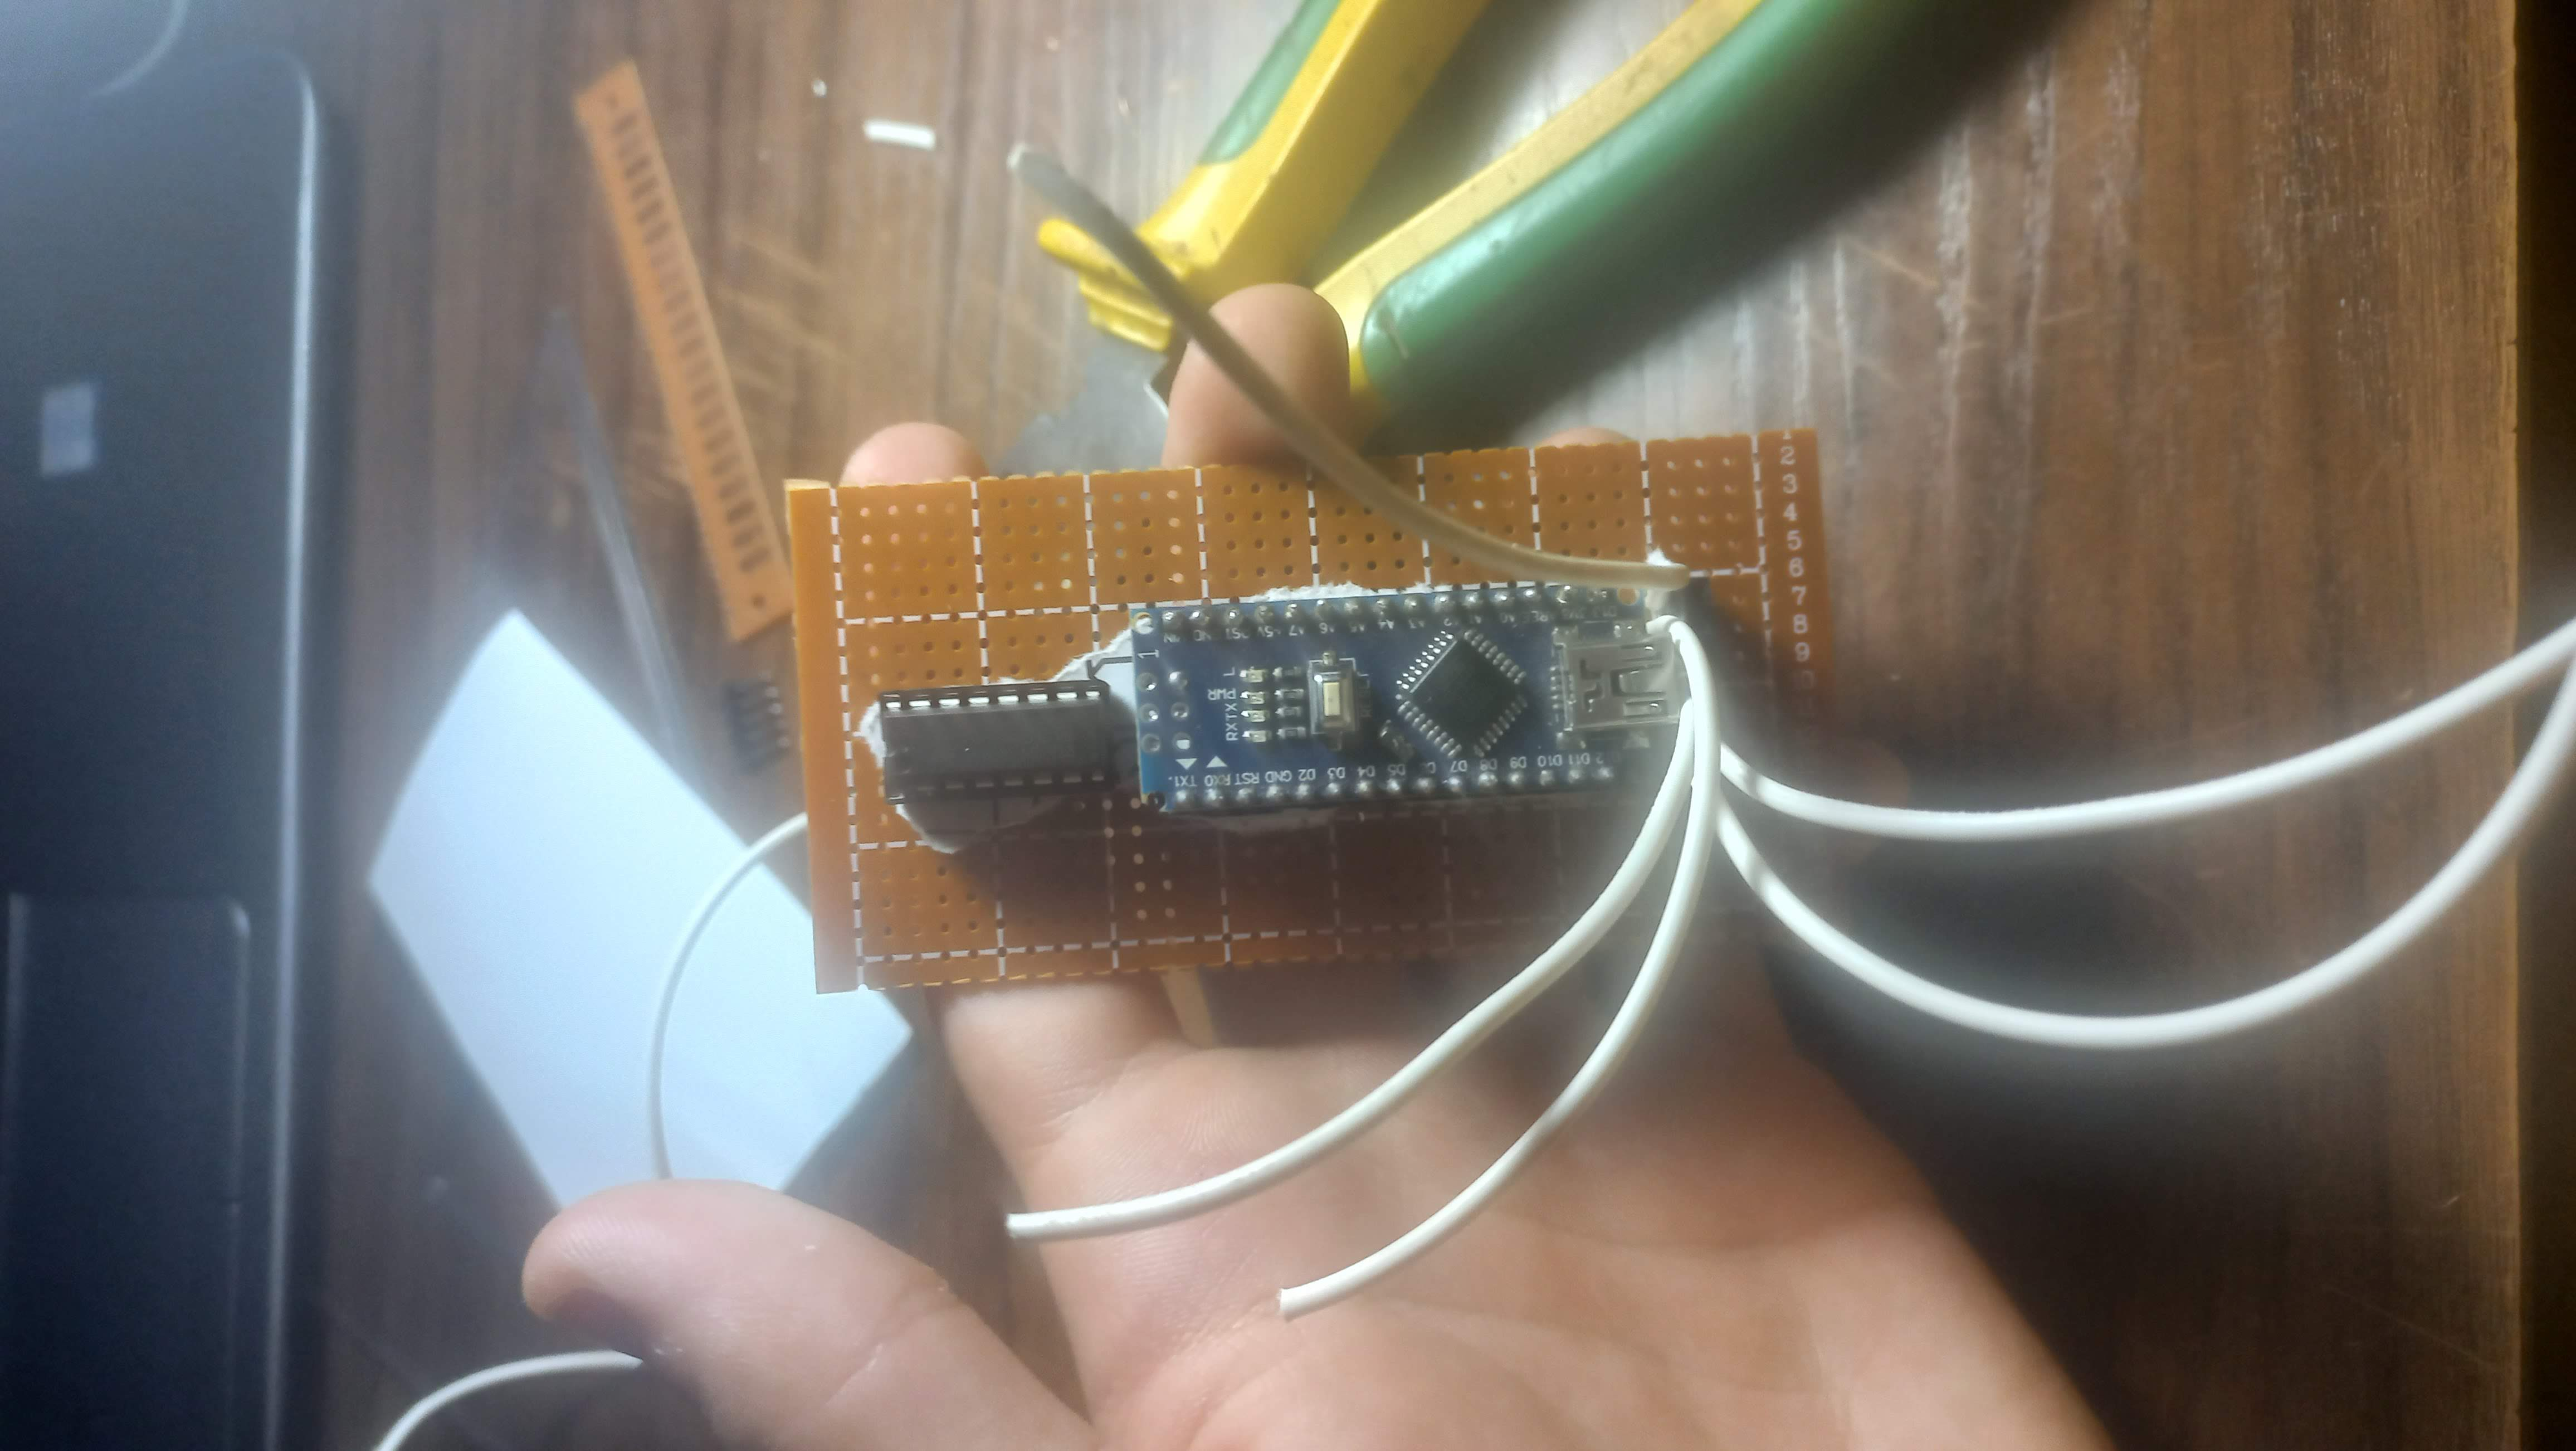
\includegraphics[height=\textwidth]{assets/realisation/2.jpg}}
    \end{subfigure}
    \hfill
    \begin{subfigure}[m]{.23\linewidth}
        \centering
        \rotatebox[origin=c]{-90}{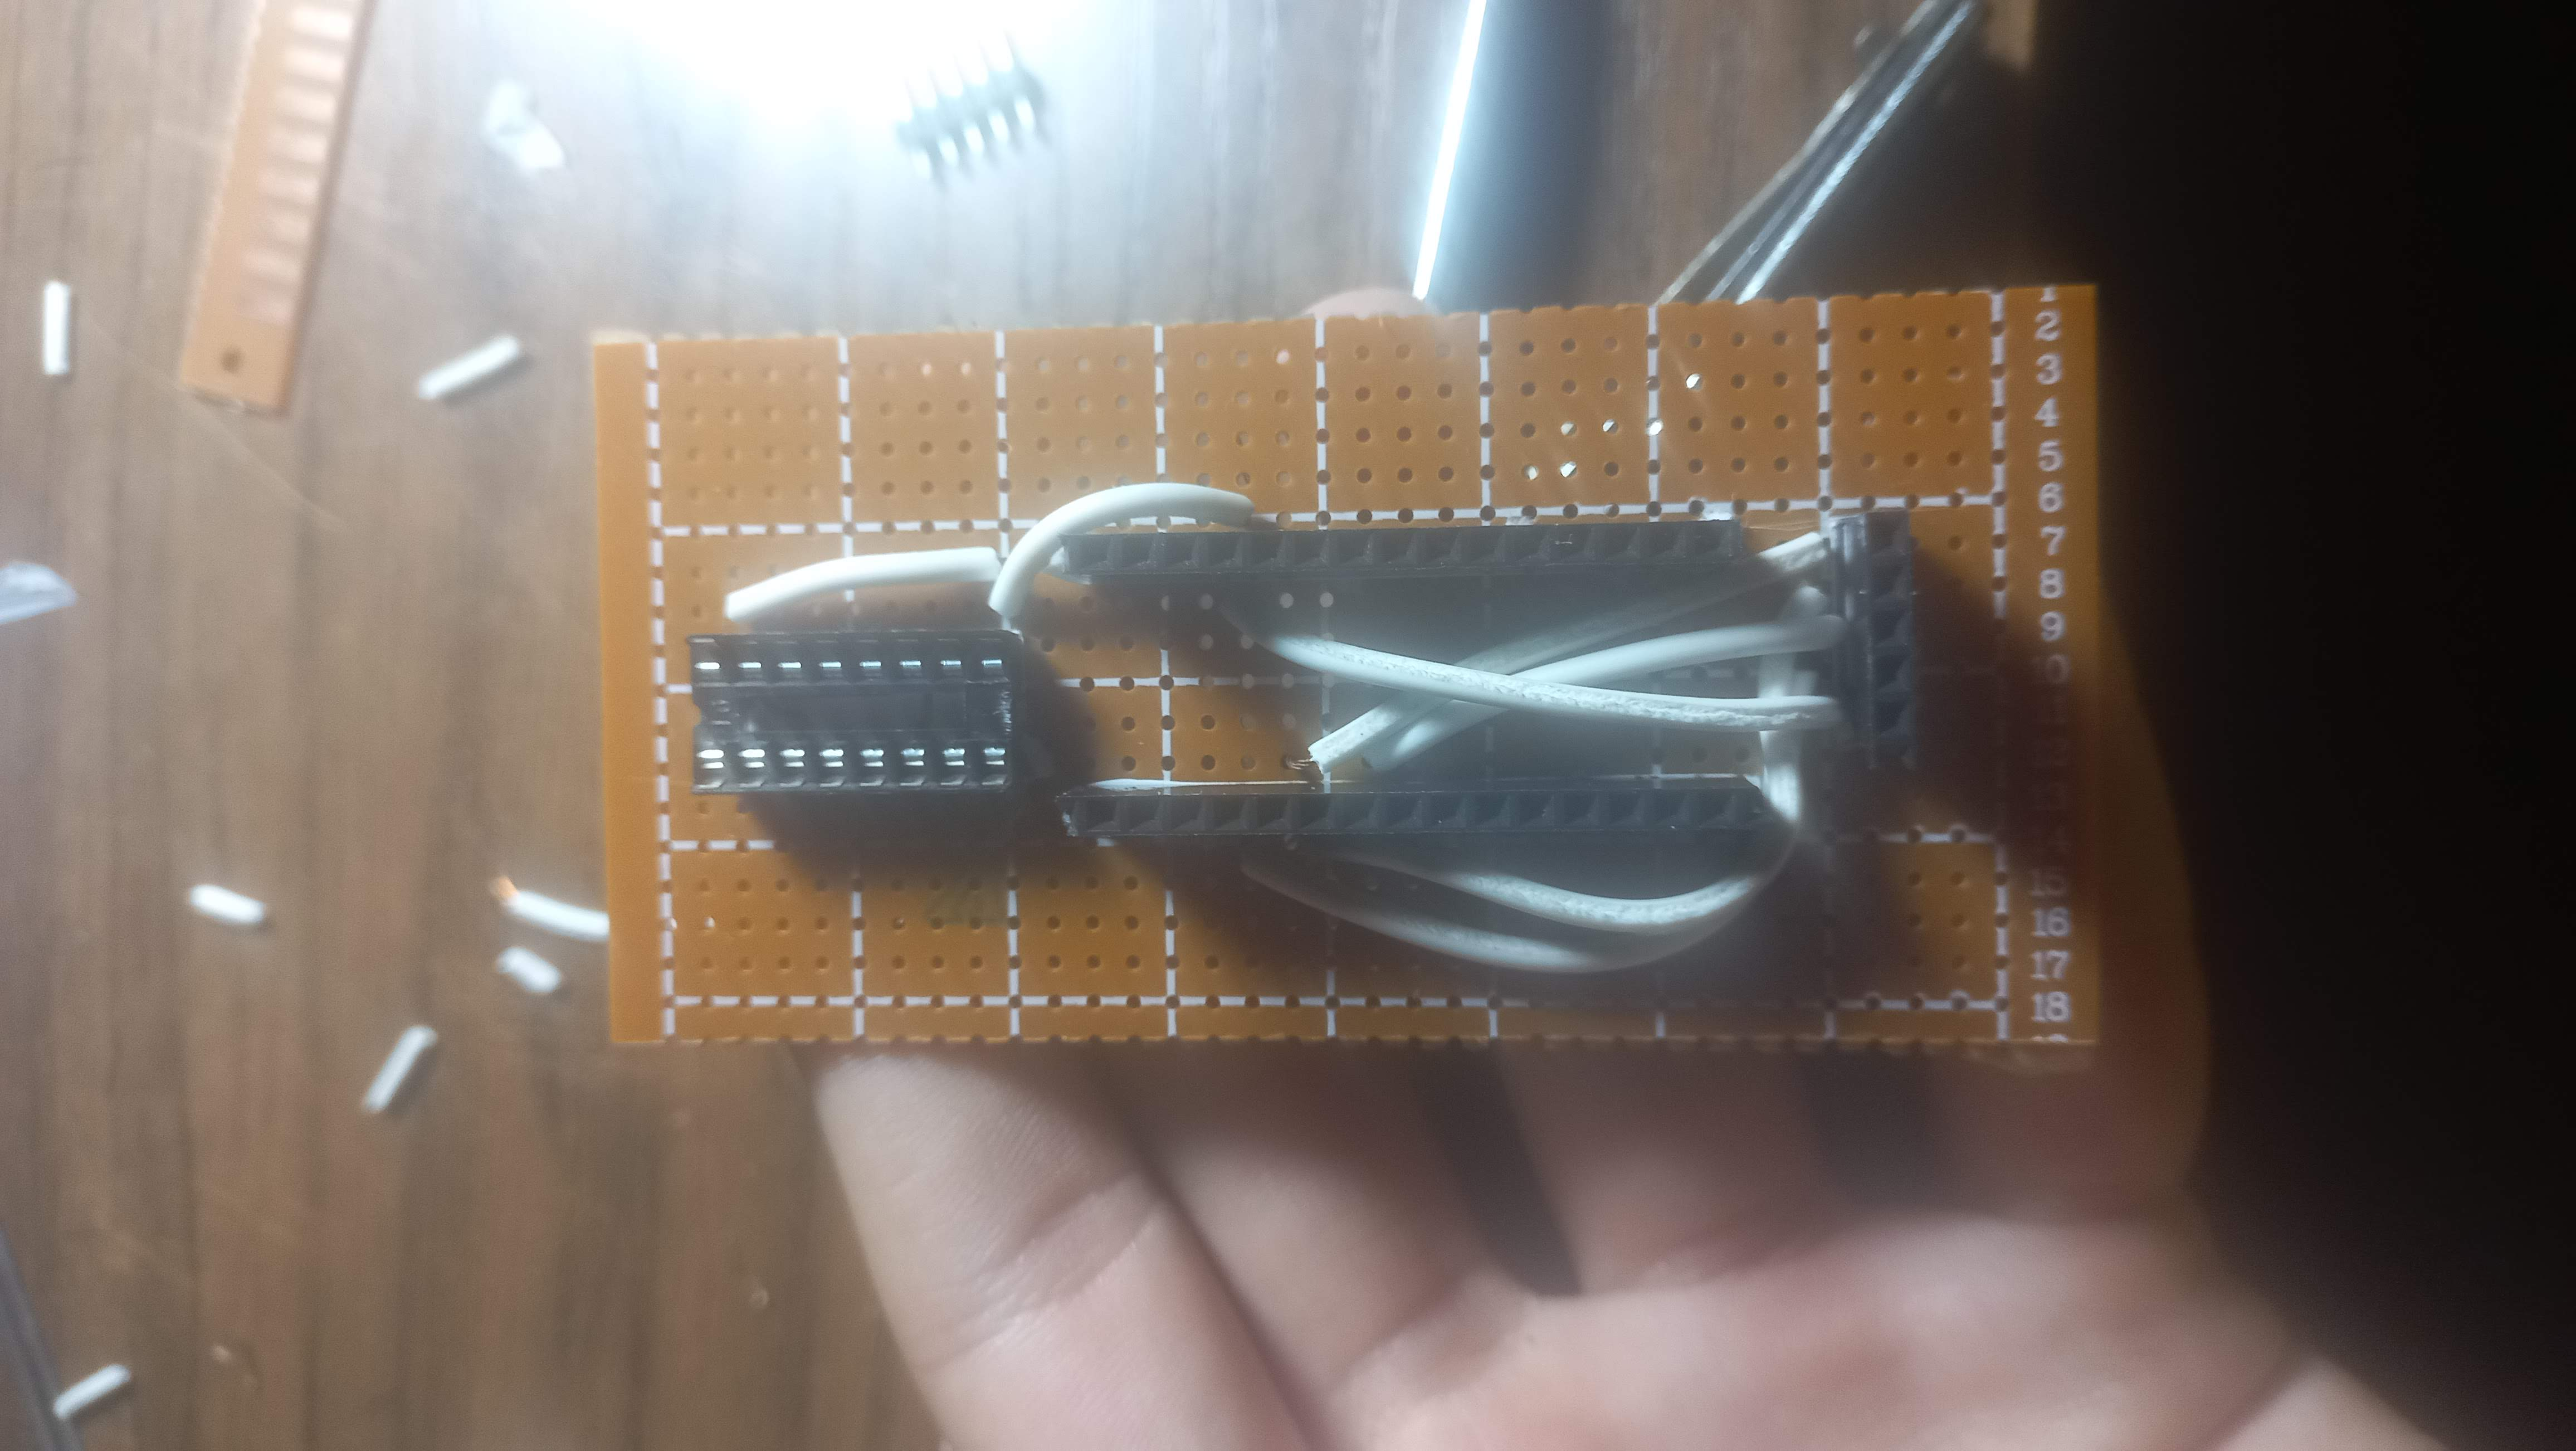
\includegraphics[height=\textwidth]{assets/realisation/3.jpg}}
    \end{subfigure}
    \hfill
    \begin{subfigure}[m]{.23\linewidth}
        \centering
        \rotatebox[origin=c]{-90}{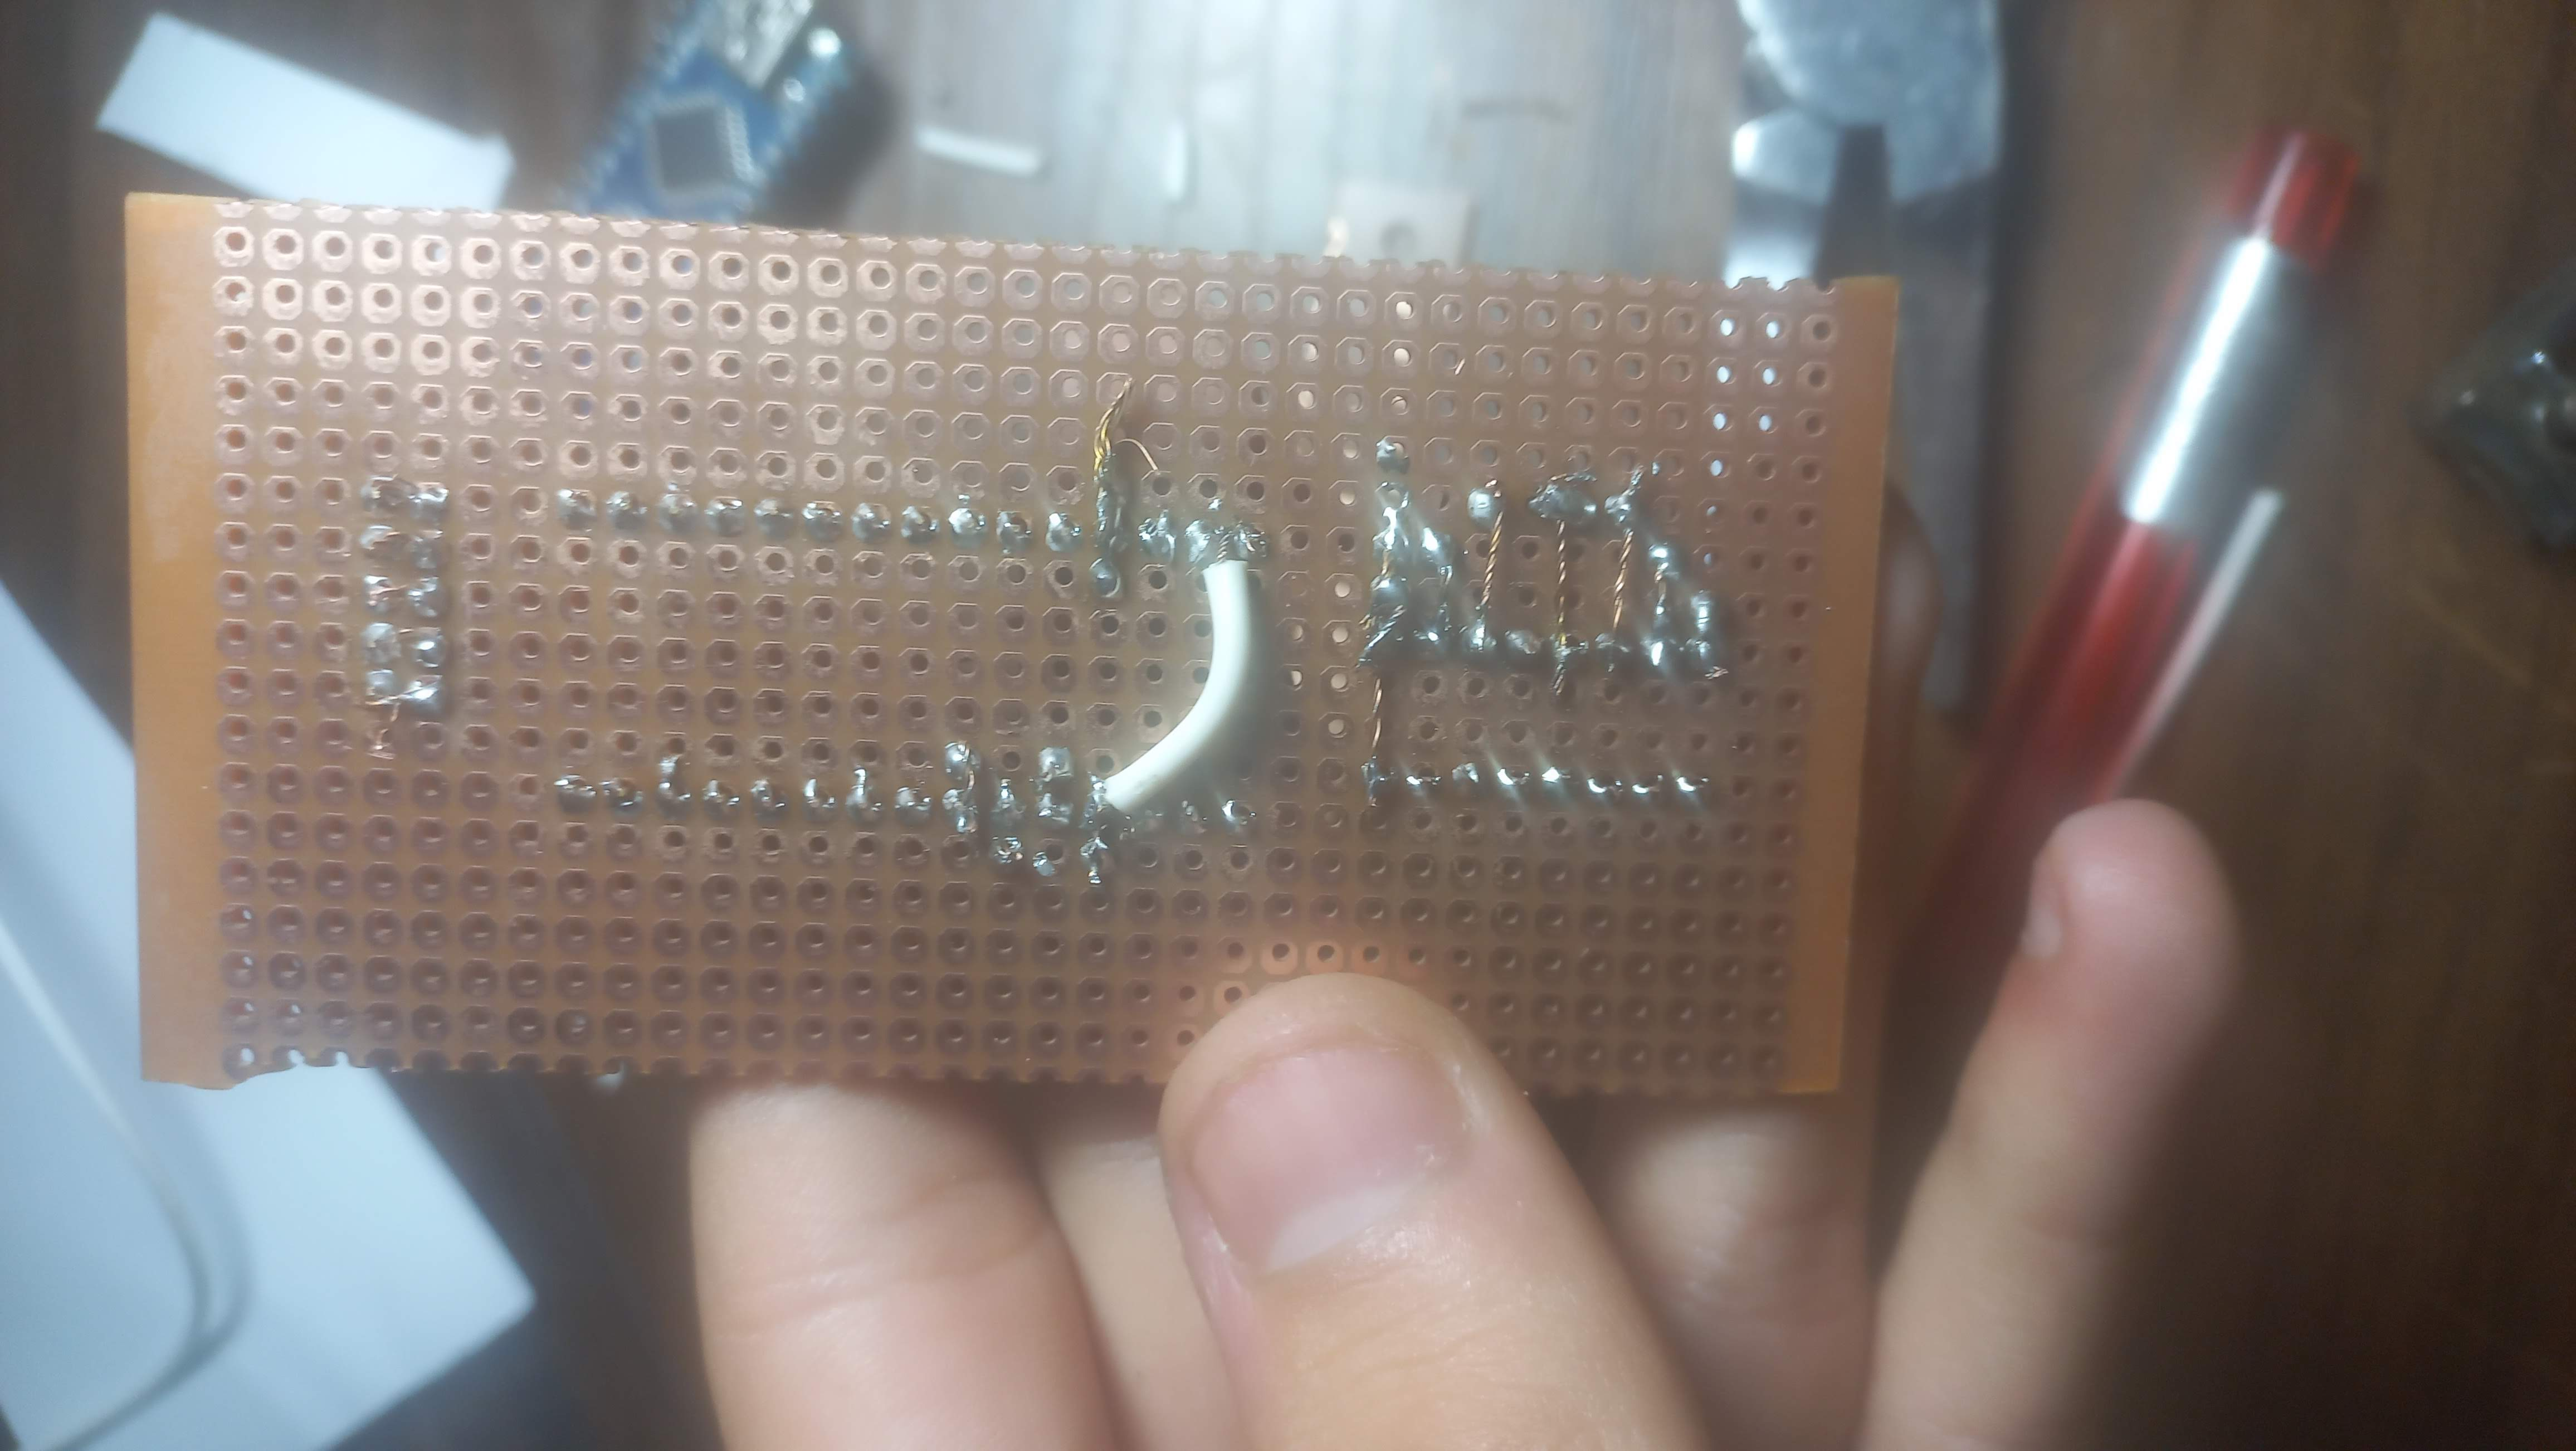
\includegraphics[height=\textwidth]{assets/realisation/4.jpg}}
    \end{subfigure}
    \caption{La réalisation du circuit d'Arduino}
\end{figure}

\FloatBarrier

\section{L'impression 3D}
L'impression du carcasse de la canne est sous-traitée chez la société \textbf{Deutsche Print Solution Design}

\begin{figure}[!htbp]
    \centering
    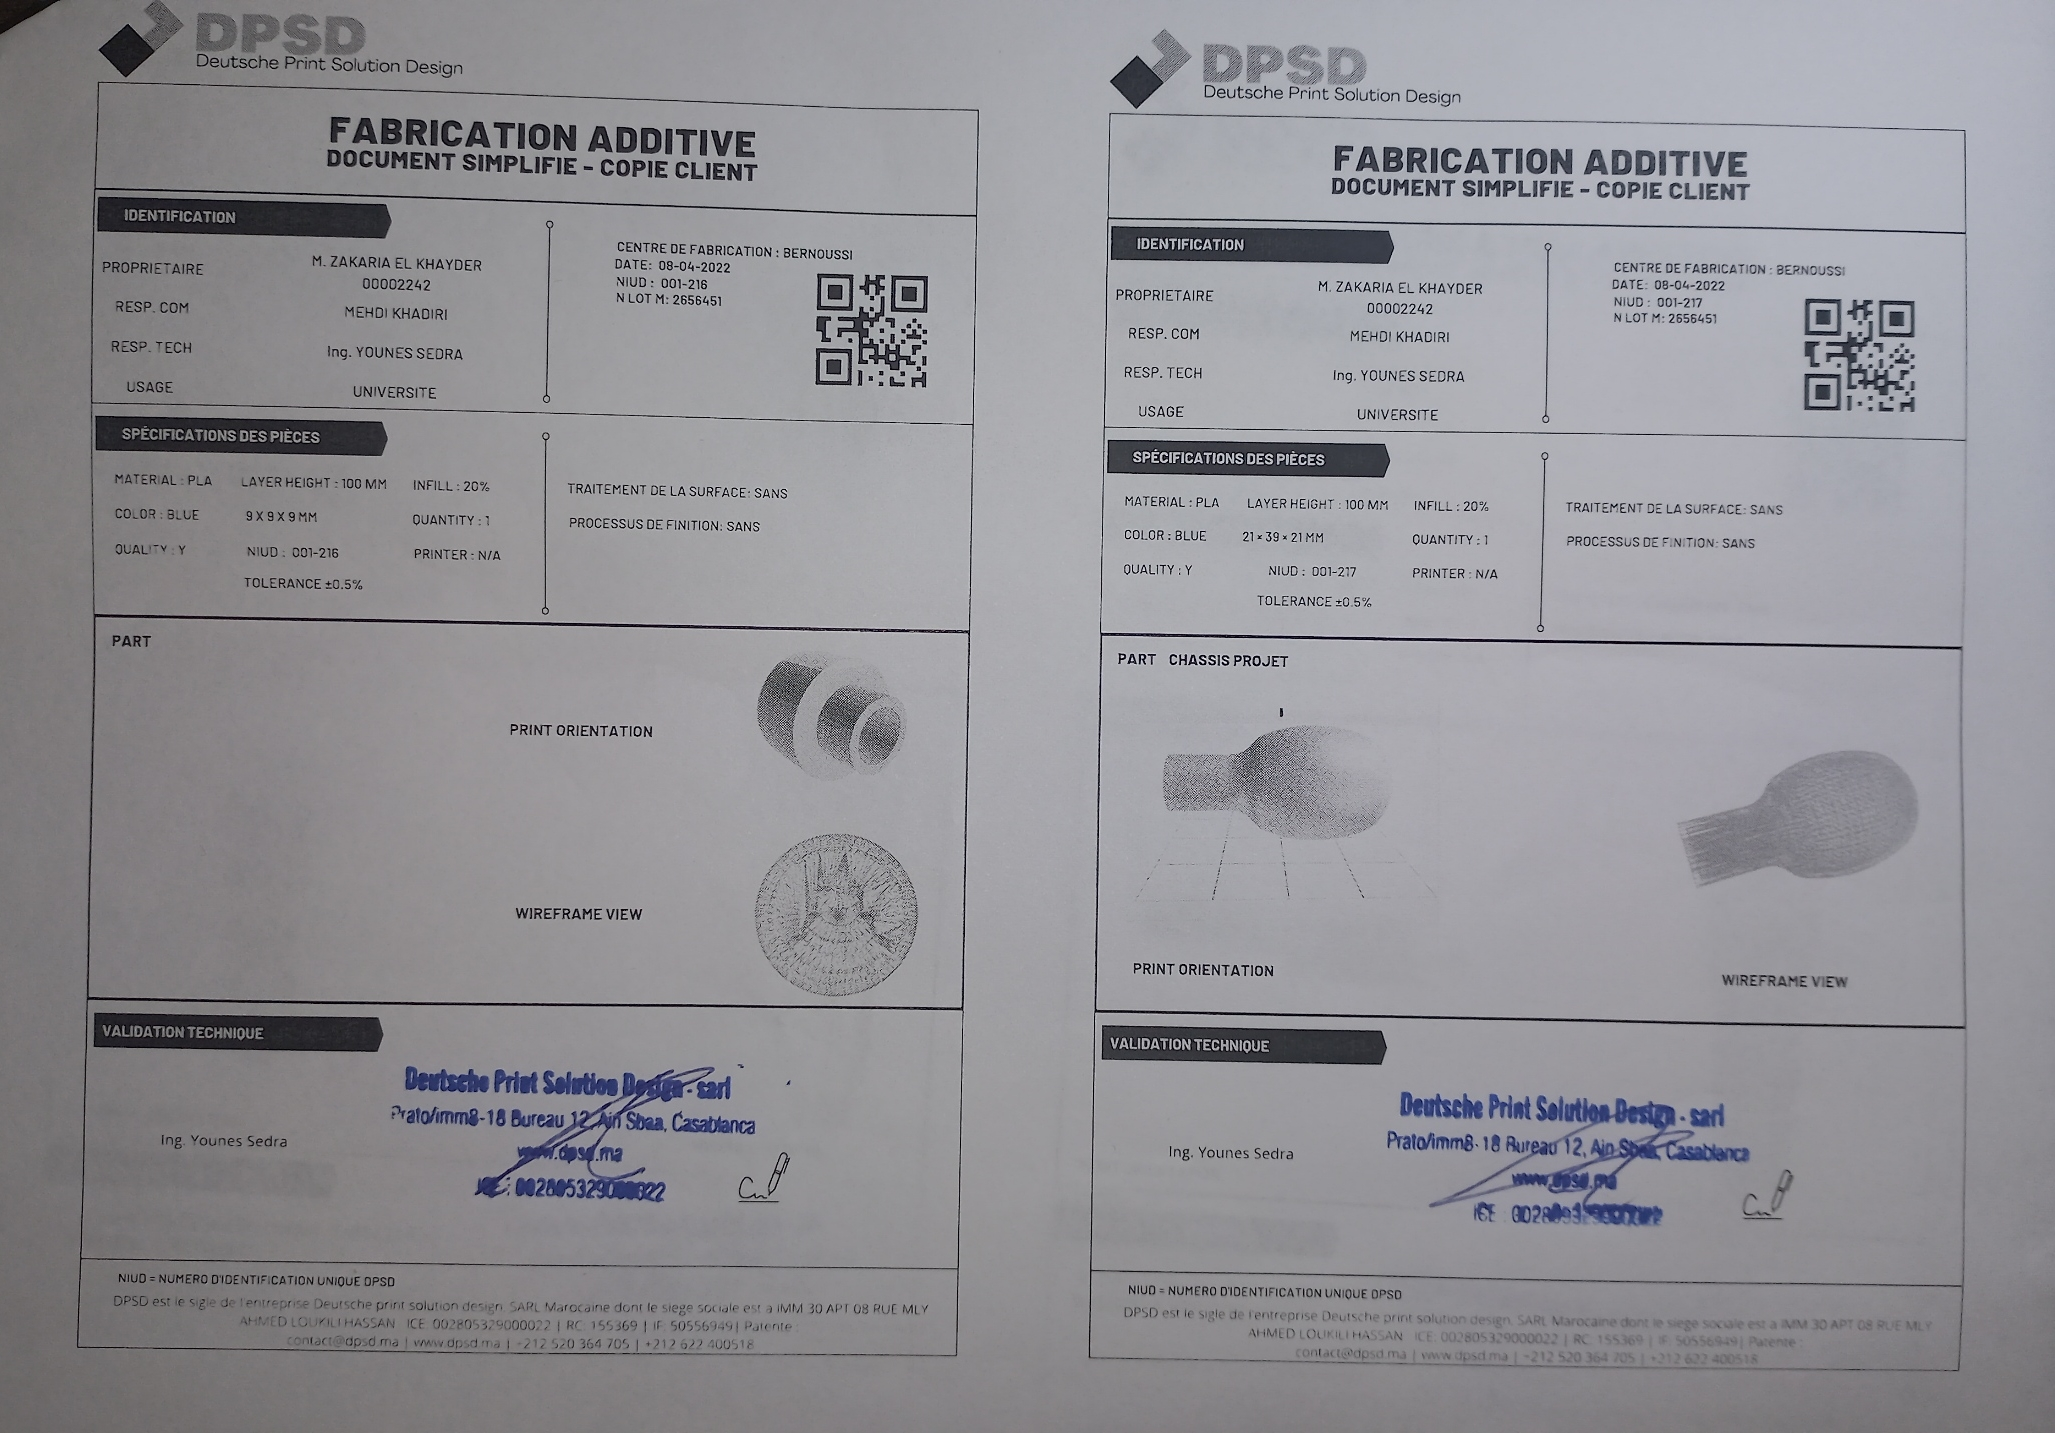
\includegraphics[height=.4\textheight]{assets/realisation/dpsd/1.jpg}
\end{figure}

\begin{figure}[!htbp]
    \centering
    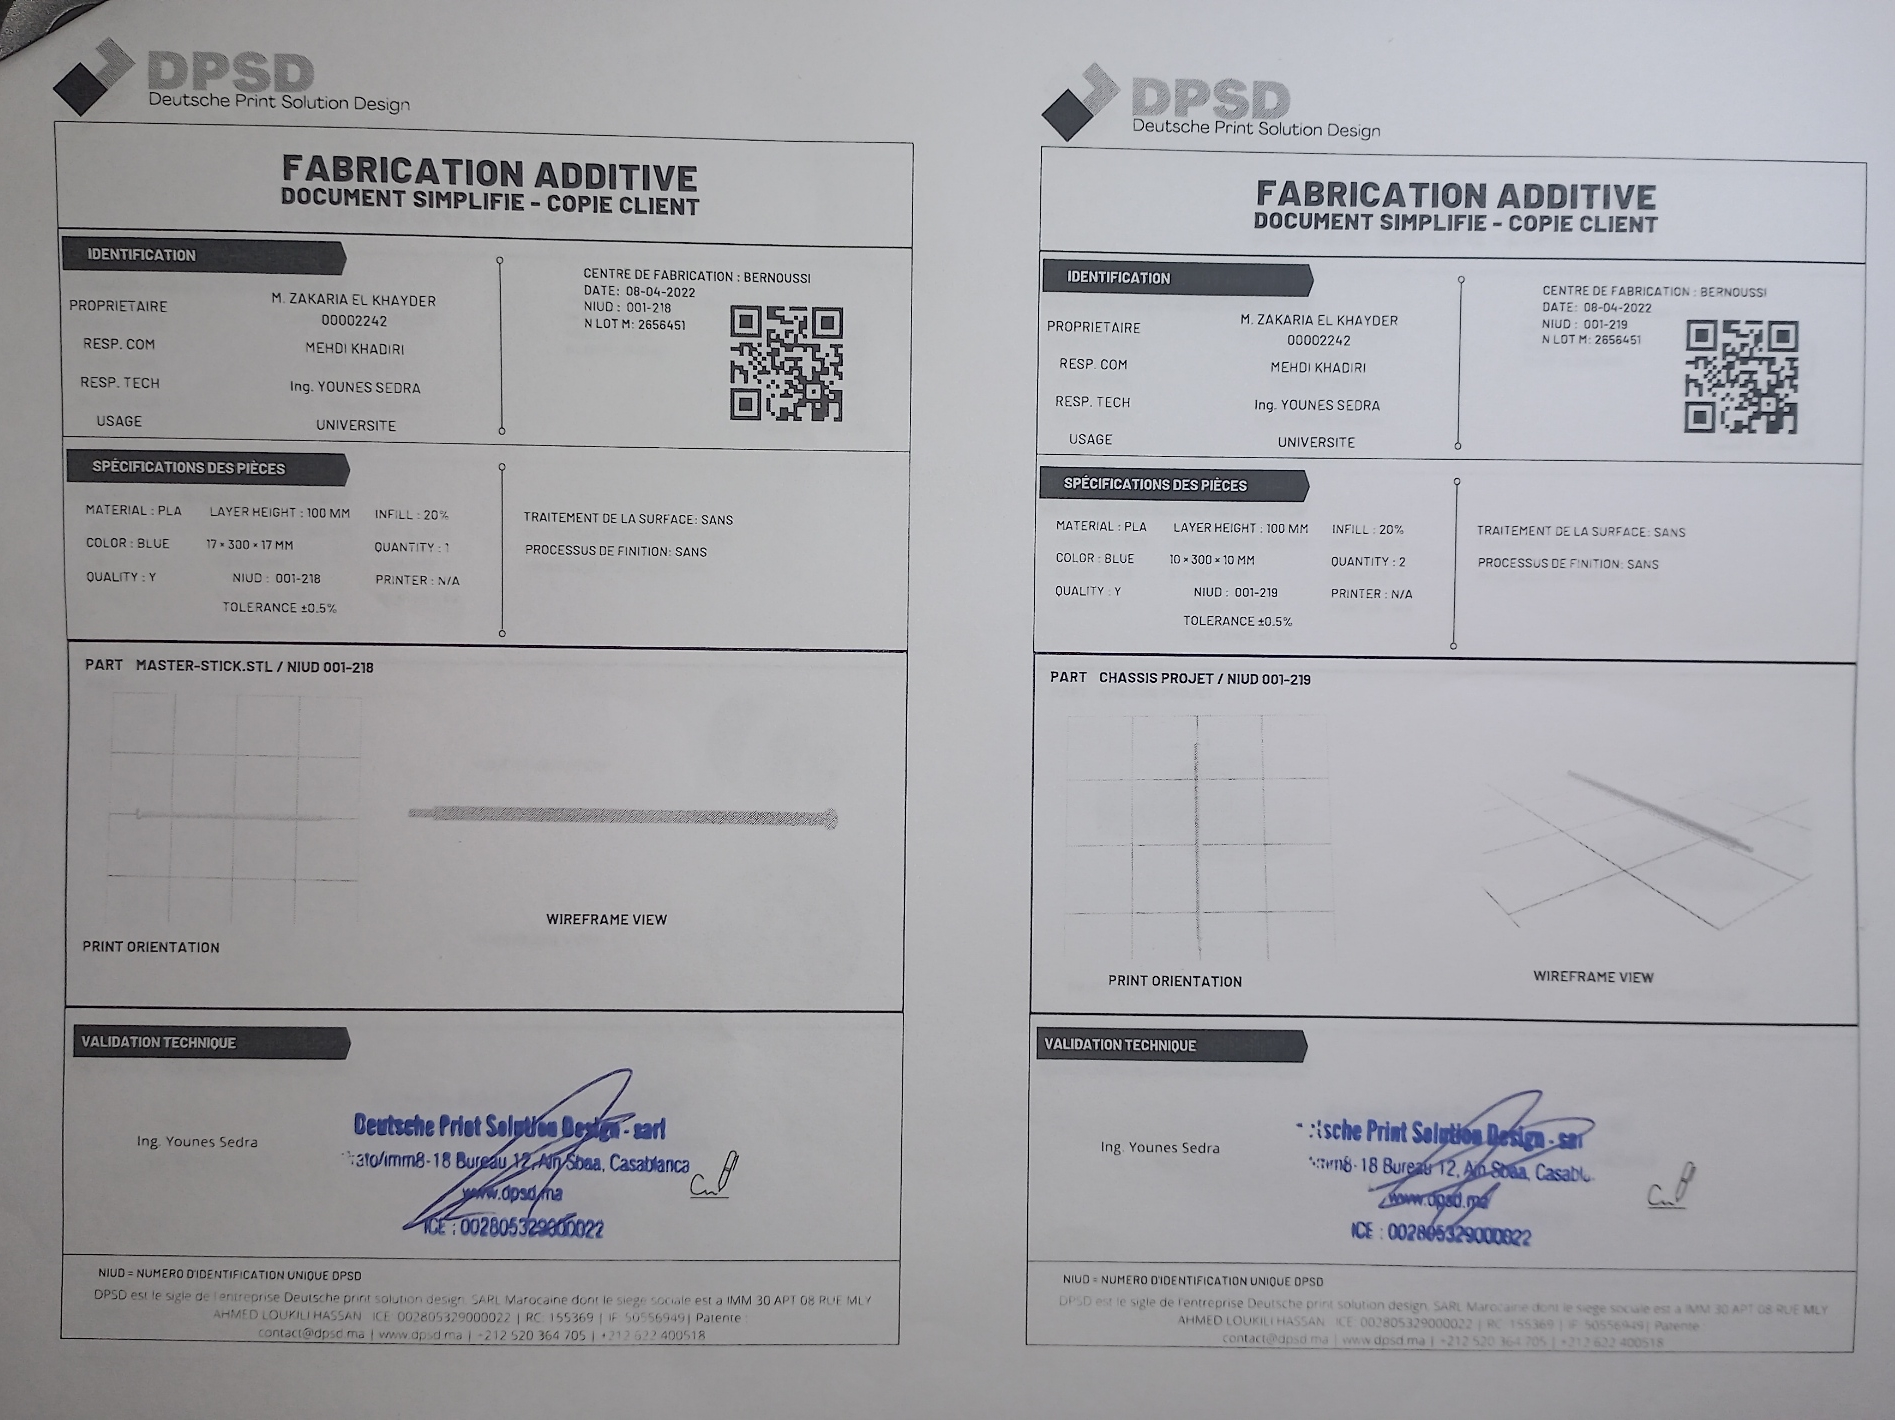
\includegraphics[height=.4\textheight]{assets/realisation/dpsd/2.jpg}
\end{figure}

\begin{figure}[!htbp]
    \centering
    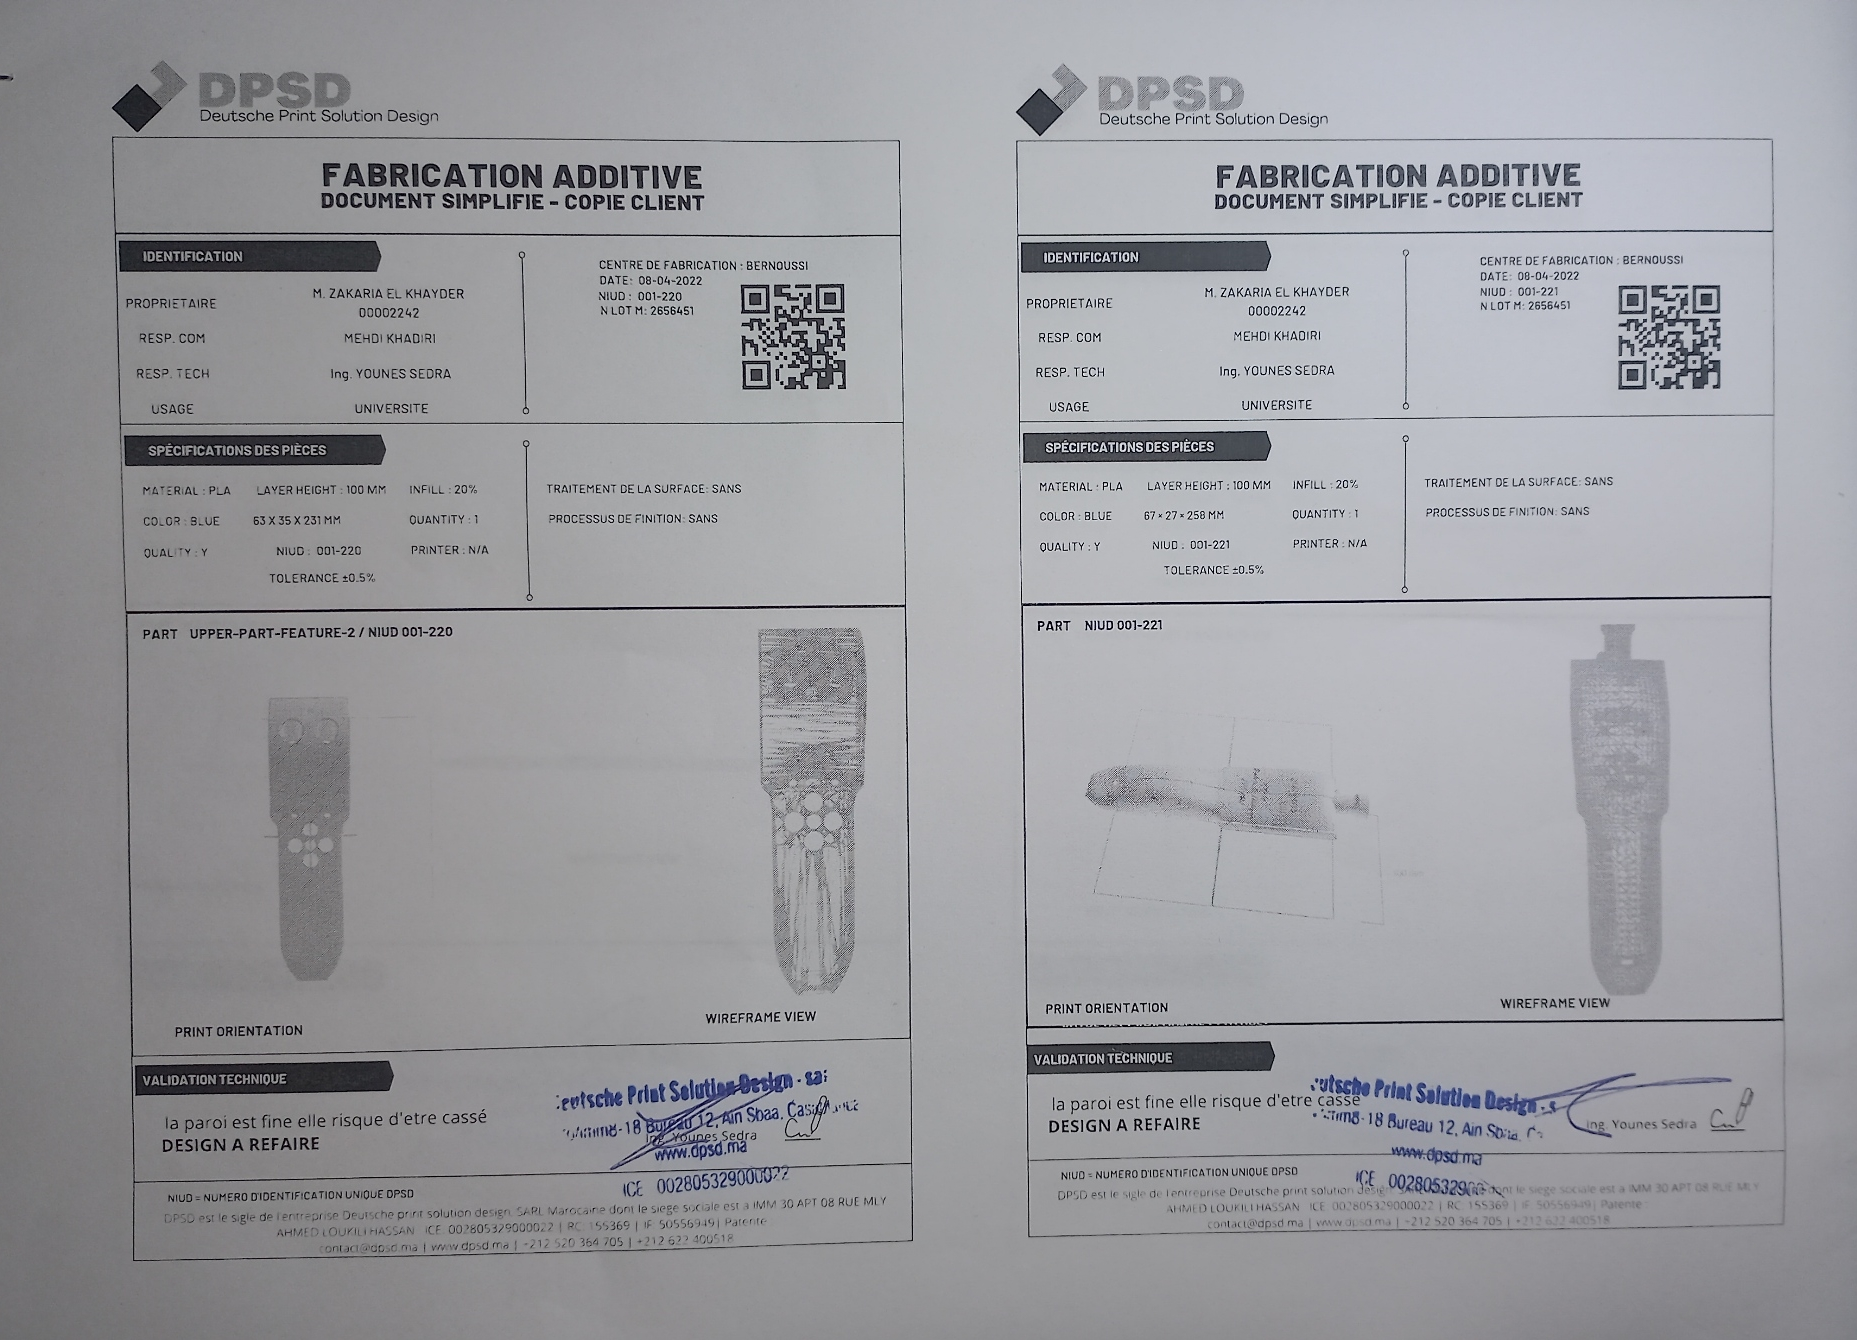
\includegraphics[height=.4\textheight]{assets/realisation/dpsd/3.jpg}
    \caption{Fiches de la fabrication additive}
\end{figure}

\FloatBarrier

\section{Le coût du projet}

\bgroup
\def\arraystretch{1.5}%
\begin{table}[!htbp]
    \centering
    \begin{tabular}{|C{6cm}|C{2cm}|C{4cm}|}
        \hline
        \verb|Article| & \verb|Nombre| & \verb|Prix total| \\
        \hline
        Pilote des moteurs L293 & 2 & 35DH \\
        \hline
        Les boutons & 6 & 27DH \\
        \hline
        Les broches & 27 & 45DH \\
        \hline
        Les fils & 40 & 45DH \\
        \hline
        Plaque de soudage & 1 & 12DH \\
        \hline
        Cables & 1 & 8DH \\
        \hline
        L'impression 3D & - & 420DH \\
        \hline
    \end{tabular}
    \caption{Les charges pour la réalisation du projet}
\end{table}
\egroup

Coût total du projet: 592DH